
\chapter{分析所使用的数据和触发列表}\label{app:data_lists}

\section{分析所使用的数据列表}

表格~\ref{tab:datasets_data_16postVFP}、\ref{tab:datasets_data_16preVFP}、\ref{tab:datasets_data_17}、\ref{tab:datasets_data_18}分别列出了本分析所使用的数据样本。表格~\ref{tab:sig_sample}列出了本分析中使用的所有信号样本,初始散射截面被设定为0.1~\si{pb};表格~\ref{tab:bkg_sample}列出了本分析中所使用的本底样本以及对应的散射截面。

\begin{table}[h]
\scriptsize
\centering
\bicaption{\quad \centering 使用的2016年post-VFP运行期间的数据。}{\quad \centering Datasets used in Run 2016 post-VFP.}
\begin{tabular}{l}
\hline
/DoubleEG/Run2016F-UL2016\_MiniAODv2-v1/MINIAOD \\
/DoubleEG/Run2016G-UL2016\_MiniAODv2-v1/MINIAOD \\
/DoubleEG/Run2016H-UL2016\_MiniAODv2-v1/MINIAOD \\
\hline
/DoubleMuon/Run2016F-UL2016\_MiniAODv2-v1/MINIAOD \\
/DoubleMuon/Run2016G-UL2016\_MiniAODv2-v1/MINIAOD \\
/DoubleMuon/Run2016H-UL2016\_MiniAODv2-v2/MINIAOD \\
\hline
/MuonEG/Run2016F-UL2016\_MiniAODv2-v2/MINIAOD \\
/MuonEG/Run2016G-UL2016\_MiniAODv2-v2/MINIAOD \\
/MuonEG/Run2016H-UL2016\_MiniAODv2-v2/MINIAOD \\
\hline
/SingleElectron/Run2016F-UL2016\_MiniAODv2-v2/MINIAOD \\
/SingleElectron/Run2016G-UL2016\_MiniAODv2-v2/MINIAOD \\
/SingleElectron/Run2016H-UL2016\_MiniAODv2-v2/MINIAOD \\
\hline
/SingleMuon/Run2016F-UL2016\_MiniAODv2-v2/MINIAOD \\
/SingleMuon/Run2016G-UL2016\_MiniAODv2-v2/MINIAOD \\
/SingleMuon/Run2016H-UL2016\_MiniAODv2-v2/MINIAOD \\
\hline
\end{tabular}
\small
\label{tab:datasets_data_16postVFP}
\end{table}

\begin{table}[h]
\scriptsize
    \centering
    \bicaption{\quad \centering 使用的2016年pre-VFP(又称为APV)运行期间的数据。}{\quad \centering Datasets used in Run 2016 pre-VFP (aka APV).}
    \begin{tabular}{l}
\hline %-------------------------------------------------------------
/DoubleMuon/Run2016B-ver2\_HIPM\_UL2016\_MiniAODv2-v1/MINIAO \\
/DoubleMuon/Run2016C-HIPM\_UL2016\_MiniAODv2-v1/MINIAOD \\
/DoubleMuon/Run2016D-HIPM\_UL2016\_MiniAODv2-v1/MINIAOD \\
/DoubleMuon/Run2016E-HIPM\_UL2016\_MiniAODv2-v1/MINIAOD \\
/DoubleMuon/Run2016F-HIPM\_UL2016\_MiniAODv2-v1/MINIAOD \\
\hline
/DoubleEG/Run2016B-ver2\_HIPM\_UL2016\_MiniAODv2-v3/MINIAOD \\
/DoubleEG/Run2016C-HIPM\_UL2016\_MiniAODv2-v1/MINIAOD  \\
/DoubleEG/Run2016D-HIPM\_UL2016\_MiniAODv2-v1/MINIAOD \\
/DoubleEG/Run2016E-HIPM\_UL2016\_MiniAODv2-v1/MINIAOD \\
/DoubleEG/Run2016F-HIPM\_UL2016\_MiniAODv2-v1/MINIAOD \\
\hline
/MuonEG/Run2016B-ver2\_HIPM\_UL2016\_MiniAODv2-v2/MINIAOD \\
/MuonEG/Run2016C-HIPM\_UL2016\_MiniAODv2-v2/MINIAOD \\
/MuonEG/Run2016D-HIPM\_UL2016\_MiniAODv2-v2/MINIAOD \\
/MuonEG/Run2016E-HIPM\_UL2016\_MiniAODv2-v2/MINIAOD \\
/MuonEG/Run2016F-HIPM\_UL2016\_MiniAODv2-v2/MINIAOD \\
\hline
/SingleElectron/Run2016B-ver2\_HIPM\_UL2016\_MiniAODv2-v2/MINIAOD \\
/SingleElectron/Run2016C-HIPM\_UL2016\_MiniAODv2-v2/MINIAOD \\
/SingleElectron/Run2016D-HIPM\_UL2016\_MiniAODv2-v2/MINIAOD \\
/SingleElectron/Run2016E-HIPM\_UL2016\_MiniAODv2-v2/MINIAOD \\
/SingleElectron/Run2016F-HIPM\_UL2016\_MiniAODv2-v2/MINIAOD \\
\hline
/SingleMuon/Run2016B-ver2\_HIPM\_UL2016\_MiniAODv2-v2/MINIAOD \\
/SingleMuon/Run2016C-HIPM\_UL2016\_MiniAODv2-v2/MINIAOD \\
/SingleMuon/Run2016D-HIPM\_UL2016\_MiniAODv2-v2/MINIAOD \\
/SingleMuon/Run2016E-HIPM\_UL2016\_MiniAODv2-v2/MINIAOD \\
/SingleMuon/Run2016F-HIPM\_UL2016\_MiniAODv2-v2/MINIAOD \\
\hline
\end{tabular}
\small
    \label{tab:datasets_data_16preVFP}
\end{table}

\begin{table}[h]
\scriptsize
    \centering
    \bicaption{\quad \centering 使用的2017年运行期间的数据。}{\quad \centering Datasets used in Run 2017.}
    \begin{tabular}{l}
\hline %-------------------------------------------------------------
/DoubleEG/Run2017B-UL2017\_MiniAODv2-v1/MINIAOD \\
/DoubleEG/Run2017C-UL2017\_MiniAODv2-v2/MINIAOD \\
/DoubleEG/Run2017D-UL2017\_MiniAODv2-v1/MINIAOD \\
/DoubleEG/Run2017E-UL2017\_MiniAODv2-v1/MINIAOD \\
/DoubleEG/Run2017F-UL2017\_MiniAODv2-v2/MINIAOD \\
\hline
/DoubleMuon/Run2017B-UL2017\_MiniAODv2-v1/MINIAOD \\
/DoubleMuon/Run2017C-UL2017\_MiniAODv2-v1/MINIAOD \\
/DoubleMuon/Run2017D-UL2017\_MiniAODv2-v1/MINIAOD \\
/DoubleMuon/Run2017E-UL2017\_MiniAODv2-v2/MINIAOD \\
/DoubleMuon/Run2017F-UL2017\_MiniAODv2-v1/MINIAOD \\
\hline
/MuonEG/Run2017B-UL2017\_MiniAODv2-v1/MINIAOD \\
/MuonEG/Run2017C-UL2017\_MiniAODv2-v1/MINIAOD \\
/MuonEG/Run2017D-UL2017\_MiniAODv2-v1/MINIAOD \\
/MuonEG/Run2017E-UL2017\_MiniAODv2-v1/MINIAOD \\
/MuonEG/Run2017F-UL2017\_MiniAODv2-v1/MINIAOD \\
\hline
/SingleMuon/Run2017B-UL2017\_MiniAODv2-v1/MINIAOD \\
/SingleMuon/Run2017C-UL2017\_MiniAODv2-v1/MINIAOD \\
/SingleMuon/Run2017D-UL2017\_MiniAODv2-v1/MINIAOD \\
/SingleMuon/Run2017E-UL2017\_MiniAODv2-v1/MINIAOD \\
/SingleMuon/Run2017F-UL2017\_MiniAODv2-v1/MINIAOD \\
\hline
        \end{tabular}
\small
    \label{tab:datasets_data_17}
\end{table}


\begin{table}[h]
\scriptsize
    \centering
    \bicaption{\quad \centering 使用的2018年运行期间的数据。}{\quad \centering Datasets used in Run 2018.}
    \begin{tabular}{l}
\hline %-------------------------------------------------------------
/SingleMuon/Run2018A-UL2018\_MiniAODv2-v3/MINIAOD \\
/SingleMuon/Run2018B-UL2018\_MiniAODv2-v2/MINIAOD \\
/SingleMuon/Run2018C-UL2018\_MiniAODv2-v2/MINIAOD \\
/SingleMuon/Run2018D-UL2018\_MiniAODv2-v3/MINIAOD \\
\hline
/EGamma/Run2018A-UL2018\_MiniAODv2-v1/MINIAOD \\
/EGamma/Run2018B-UL2018\_MiniAODv2-v1/MINIAOD \\
/EGamma/Run2018C-UL2018\_MiniAODv2-v1/MINIAOD \\
/EGamma/Run2018D-UL2018\_MiniAODv2-v1/MINIAOD \\
\hline
/MuonEG/Run2018A-UL2018\_MiniAODv2-v1/MINIAOD \\
/MuonEG/Run2018B-UL2018\_MiniAODv2-v1/MINIAOD \\
/MuonEG/Run2018C-UL2018\_MiniAODv2-v1/MINIAOD \\
/MuonEG/Run2018D-UL2018\_MiniAODv2-v1/MINIAOD \\
\hline
/DoubleMuon/Run2018A-UL2018\_MiniAODv2-v1/MINIAOD \\
/DoubleMuon/Run2018B-UL2018\_MiniAODv2-v1/MINIAOD \\
/DoubleMuon/Run2018C-UL2018\_MiniAODv2-v1/MINIAOD \\
/DoubleMuon/Run2018D-UL2018\_MiniAODv2-v1/MINIAOD \\
\hline
     \end{tabular}
\small
    \label{tab:datasets_data_18}
\end{table}


\begin{table}
\begin{scriptsize}
    \centering
    \bicaption{\quad \centering 分析中使用的信号样本。}{\quad \centering Signal samples used in the analysis.}
    \resizebox{\textwidth}{!}{
    \begin{tabular}{l}
    \hline
    Dataset Name\\ \hline
    /HZaTo2l2g\_M1\_TuneCP5\_PSWeights\_13TeV-madgraph\_pythia8/[1] \\
    /HZaTo2l2g\_M2\_TuneCP5\_PSWeights\_13TeV-madgraph\_pythia8/[1] \\
    /HZaTo2l2g\_M3\_TuneCP5\_PSWeights\_13TeV-madgraph\_pythia8/[1] \\
    /HZaTo2l2g\_M4\_TuneCP5\_PSWeights\_13TeV-madgraph\_pythia8/[1] \\
    /HZaTo2l2g\_M5\_TuneCP5\_PSWeights\_13TeV-madgraph\_pythia8/[1] \\
    /HZaTo2l2g\_M6\_TuneCP5\_PSWeights\_13TeV-madgraph\_pythia8/[1] \\
    /HZaTo2l2g\_M7\_TuneCP5\_PSWeights\_13TeV-madgraph\_pythia8/[1] \\
    /HZaTo2l2g\_M8\_TuneCP5\_PSWeights\_13TeV-madgraph\_pythia8/[1] \\
    /HZaTo2l2g\_M9\_TuneCP5\_PSWeights\_13TeV-madgraph\_pythia8/[1] \\
    /HZaTo2l2g\_M10\_TuneCP5\_PSWeights\_13TeV-madgraph\_pythia8/[1] \\
    /HZaTo2l2g\_M15\_TuneCP5\_PSWeights\_13TeV-madgraph\_pythia8/[1] \\
    /HZaTo2l2g\_M20\_TuneCP5\_PSWeights\_13TeV-madgraph\_pythia8/[1] \\
    /HZaTo2l2g\_M25\_TuneCP5\_PSWeights\_13TeV-madgraph\_pythia8/[1] \\
    /HZaTo2l2g\_M30\_TuneCP5\_PSWeights\_13TeV-madgraph\_pythia8/[1] \\
    \hline
    \multicolumn{1}{l}{[1] = RunIISummer20UL16MiniAODv2-106X\_mcRun2\_asymptotic\_v17-v2/MINIAODSIM for 2016 postVFP} \\
    \multicolumn{1}{l}{[1] = RunIISummer20UL16MiniAODAPVv2-106X\_mcRun2\_asymptotic\_preVFP\_v11-v2/MINIAODSIM for 2016 preVFP} \\
    \multicolumn{1}{l}{[1] = RunIISummer20UL17MiniAODv2-106X\_mc2017\_realistic\_v9-v2/MINIAODSIM for 2017} \\
    \multicolumn{1}{l}{[1] = RunIISummer20UL18MiniAODv2-106X\_upgrade2018\_realistic\_v16\_L1v1-v2/MINIAODSIM for 2018} \\
    \end{tabular}}
    \label{tab:sig_sample}
\end{scriptsize}
\end{table}

\begin{table}
\begin{footnotesize}
    \centering
     \bicaption{\quad \centering 分析中使用的本底MC样本以及对应的散射截面。}{\quad \centering Background Monte Carlo samples and cross sections used in the analysis.}
    \resizebox{\textwidth}{!}{
    \begin{tabular}{llr}
   \hline
 Process & Dataset Name & $\sigma\cdot BR$ \\ \hline
 $Z \to \ell\ell$ + jets & /DYJetsToLL\_M-50\_TuneCP5\_13TeV-[1]-pythia8/[2] & $6435 \rm{ pb}$ \\ \hline
 \multicolumn{3}{l}{[1] = madgraphMLM for 2016 preVFP }\\
 \multicolumn{3}{l}{[1] = amcatnloFXFX for 2016 postVFP, 2017 and 2018 }\\
 \multicolumn{3}{l}{[2] = RunIISummer20UL16MiniAODv2-106X\_mcRun2\_asymptotic\_v17-v1/MINIAODSIM for 2016 postVFP }\\
 \multicolumn{3}{l}{[2] = RunIISummer20UL16MiniAODAPVv2-106X\_mcRun2\_asymptotic\_preVFP\_v11-v1/MINIAODSIM for 2016 preVFP }\\
 \multicolumn{3}{l}{[2] = RunIISummer20UL17MiniAODv2-106X\_mc2017\_realistic\_v9-v2/MINIAODSIM for 2017 }\\
 \multicolumn{3}{l}{[2] = RunIISummer20UL18MiniAODv2-106X\_upgrade2018\_realistic\_v16\_L1v1-v2/MINIAODSIM for 2018 }\\
 \end{tabular}
 }
  \label{tab:bkg_sample}
\end{footnotesize}
\end{table}

\section{分析所使用的触发列表}\label{app:trigger_lists}

表格~\ref{tab:triggerPaths_16}、~\ref{tab:triggerPaths_17}、~\ref{tab:triggerPaths_18}列出了本分析中所使用的触发。

\begin{table}[h]
\scriptsize
    \centering
    \bicaption{\quad \centering 2016年post-VFP和pre-VFP对撞数据所使用的触发路径。}{\quad \centering Trigger paths used in 2016 post-VFP and pre-VFP collision data.}
    \resizebox{\textwidth}{!}{
    \begin{tabular}{ll}
\hline %--------------------------------------------------------------------------------------------------------------------------
HLT path                      				                    & primary dataset \\
\hline %--------------------------------------------------------------------------------------------------------------------------
HLT\_Ele17\_Ele12\_CaloIdL\_TrackIdL\_IsoVL\_DZ                  & DoubleEG \\
HLT\_Ele23\_Ele12\_CaloIdL\_TrackIdL\_IsoVL\_DZ                  & DoubleEG \\
HLT\_DoubleEle33\_CaloIdL\_GsfTrkIdVL                         & DoubleEG \\
HLT\_Mu17\_TrkIsoVVL\_Mu8\_TrkIsoVVL                           & DoubleMuon \\
HLT\_Mu17\_TrkIsoVVL\_TkMu8\_TrkIsoVVL                         & DoubleMuon \\
HLT\_Mu8\_TrkIsoVVL\_Ele17\_CaloIdL\_TrackIdL\_IsoVL             & MuonEG \\
HLT\_Mu8\_TrkIsoVVL\_Ele23\_CaloIdL\_TrackIdL\_IsoVL             & MuonEG \\
HLT\_Mu17\_TrkIsoVVL\_Ele12\_CaloIdL\_TrackIdL\_IsoVL            & MuonEG \\
HLT\_Mu23\_TrkIsoVVL\_Ele12\_CaloIdL\_TrackIdL\_IsoVL            & MuonEG \\
HLT\_Mu23\_TrkIsoVVL\_Ele8\_CaloIdL\_TrackIdL\_IsoVL             & MuonEG \\
HLT\_Ele25\_eta2p1\_WPTight                                   & SingleElectron \\
HLT\_Ele27\_WPTight                                          & SingleElectron \\
HLT\_Ele27\_eta2p1\_WPLoose\_Gsf                               & SingleElectron \\
HLT\_IsoMu20 OR HLT\_IsoTkMu20                               & SingleMuon \\
HLT\_IsoMu22 OR HLT\_IsoTkMu22                               & SingleMuon \\
HLT\_IsoMu24 OR HLT\_IsoTkMu24                               & SingleMuon \\
\hline %--------------------------------------------------------------------------------------------------------------------------
    \end{tabular}
    }
\small
    \label{tab:triggerPaths_16}
\end{table}

\begin{table}[h]
\scriptsize
    \centering
    \bicaption{\quad \centering 2017年对撞数据所使用的触发路径。}{\quad \centering Trigger paths used in 2017 collision data.}
    \resizebox{\textwidth}{!}{
    \begin{tabular}{ll}
\hline %--------------------------------------------------------------------------------------------------------------------------
HLT path                      				                    & primary dataset \\
\hline %--------------------------------------------------------------------------------------------------------------------------
HLT\_Ele35\_WPTight\_Gsf\_v*                                  & DoubleEG \\
HLT\_Ele38\_WPTight\_Gsf\_v*                                  & DoubleEG \\
HLT\_Ele40\_WPTight\_Gsf\_v*                                  & DoubleEG \\
HLT\_Ele23\_Ele12\_CaloIdL\_TrackIdL\_IsoVL\_v*                 & DoubleEG \\
HLT\_DoubleEle33\_CaloIdL\_MW\_v*                             & DoubleEG \\
HLT\_IsoMu27\_v*                                           & DoubleMuon \\
HLT\_Mu17\_TrkIsoVVL\_Mu8\_TrkIsoVVL\_DZ\_Mass3p8\_v*            & DoubleMuon \\
HLT\_Mu23\_TrkIsoVVL\_Ele12\_CaloIdL\_TrackIdL\_IsoVL\_v*        & DoubleMuon \\
HLT\_Mu8\_TrkIsoVVL\_Ele23\_CaloIdL\_TrackIdL\_IsoVL\_DZ\_v*      & DoubleMuon \\
HLT\_Mu12\_TrkIsoVVL\_Ele23\_CaloIdL\_TrackIdL\_IsoVL\_DZ\_v*     & DoubleMuon \\
HLT\_Mu23\_TrkIsoVVL\_Ele12\_CaloIdL\_TrackIdL\_IsoVL\_DZ\_v*     & DoubleMuon \\
\hline %--------------------------------------------------------------------------------------------------------------------------
    \end{tabular}
    }
\small
    \label{tab:triggerPaths_17}
\end{table}

\begin{table}[h]
\scriptsize
    \centering
    \bicaption{\quad \centering 2018年对撞数据所使用的触发路径。}{\quad \centering Trigger paths used in 2018 collision data.}
    \resizebox{\textwidth}{!}{
    \begin{tabular}{ll}
\hline %--------------------------------------------------------------------------------------------------------------------------
HLT path                      				                    & primary dataset \\
\hline %--------------------------------------------------------------------------------------------------------------------------
HLT\_Ele23\_Ele12\_CaloIdL\_TrackIdL\_IsoVL\_v*                         & DoubleEG \\
HLT\_DoubleEle25\_CaloIdL\_MW\_v*                                     & DoubleEG \\
HLT\_Mu17\_TrkIsoVVL\_Mu8\_TrkIsoVVL\_DZ\_Mass3p8\_v*                    & DoubleMuon \\
HLT\_Mu23\_TrkIsoVVL\_Ele12\_CaloIdL\_TrackIdL\_IsoVL\_v*                & MuonEG \\
HLT\_Mu8\_TrkIsoVVL\_Ele23\_CaloIdL\_TrackIdL\_IsoVL\_DZ\_v*              & MuonEG \\
HLT\_Mu12\_TrkIsoVVL\_Ele23\_CaloIdL\_TrackIdL\_IsoVL\_DZ\_v*             & MuonEG \\
HLT\_Ele32\_WPTight\_Gsf\_v*                                          & SingleElectron \\
HLT\_IsoMu24\_v*                                                    & SingleMuon \\
\hline %--------------------------------------------------------------------------------------------------------------------------
    \end{tabular}
    }
\small
    \label{tab:triggerPaths_18}
\end{table}

\chapter{所有质量点的信号模型}\label{app:signalModel}

\begin{figure}[htbp]
  \begin{center}
		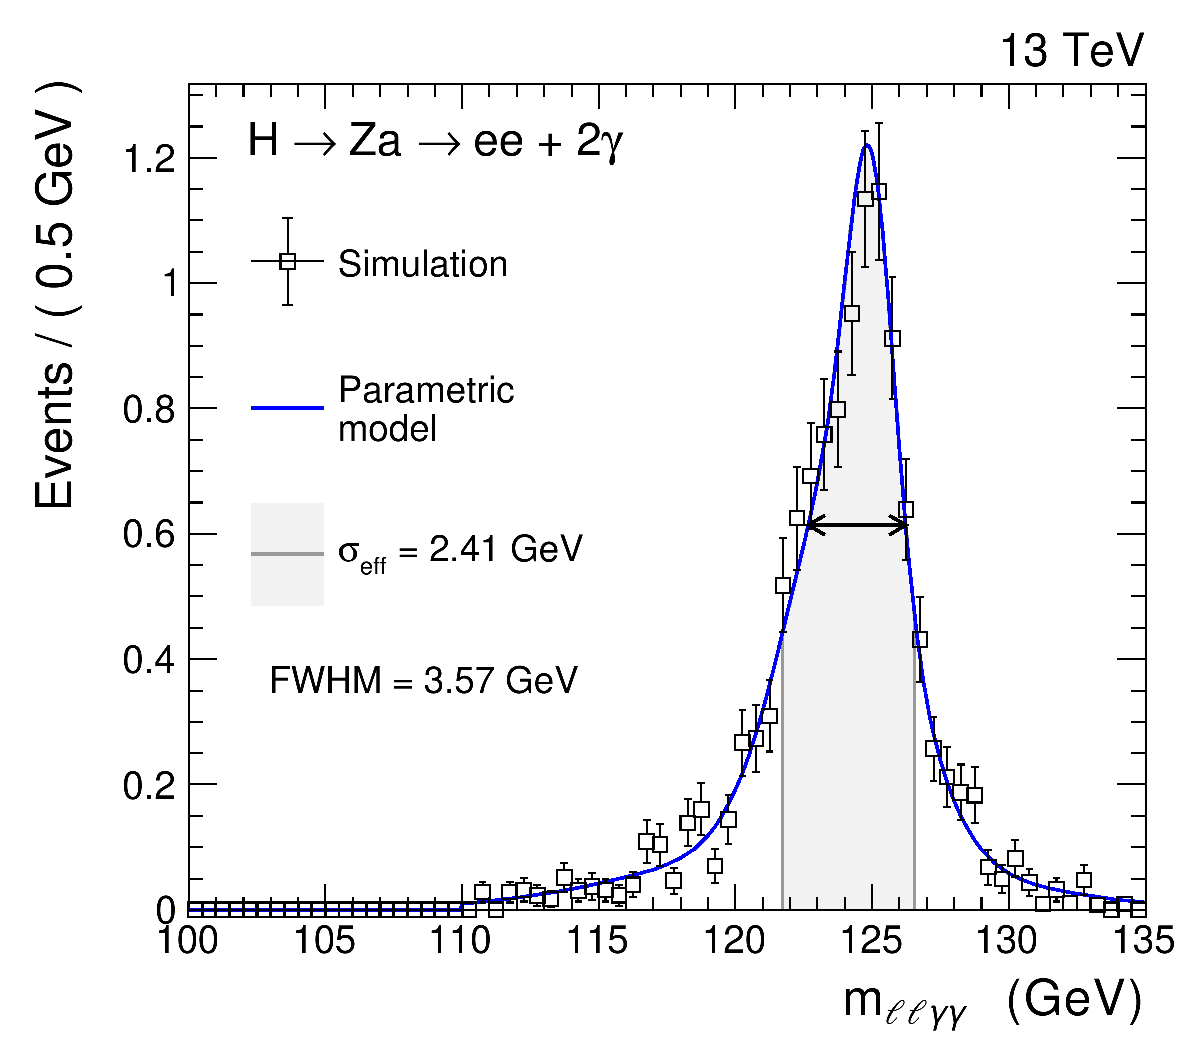
\includegraphics[width=0.5\textwidth,page=1]{figures/chapter04/sig_model/sigModel_M2_ele.pdf}
        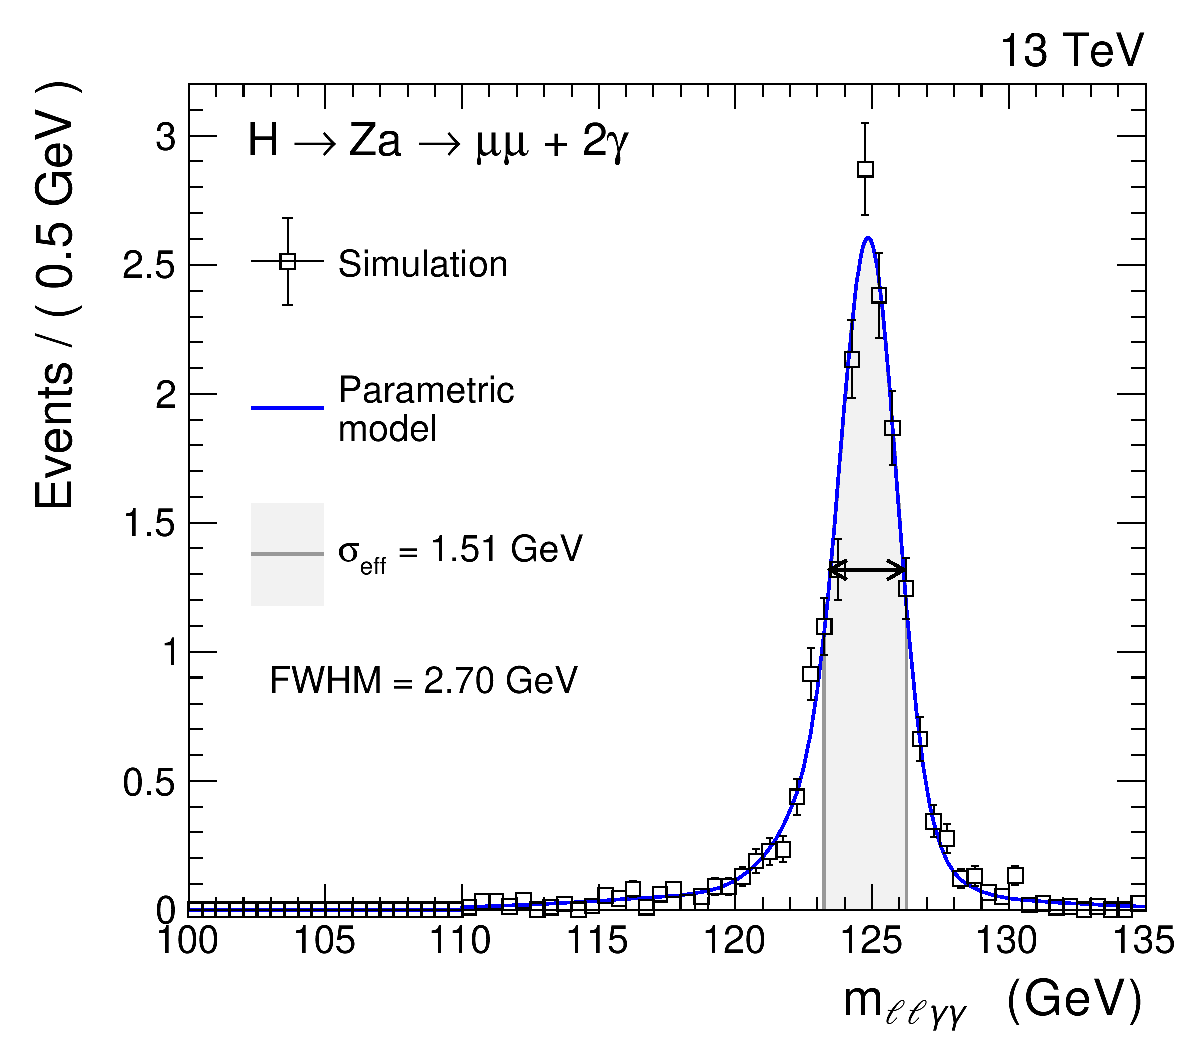
\includegraphics[width=0.5\textwidth,page=1]{figures/chapter04/sig_model/sigModel_M2_mu.pdf}
    \bicaption{\quad \centering 采用2016年post-VFP取数阶段的探测器设置,在电子(上图)和缪子(下图)道中拟合$\ma = 2~\si{GeV}$的信号事例样本的$\mllgg$分布。}{\quad \centering Fit of the $\mllgg$ distribution of signal events with $\ma = 2~\si{GeV}$ in the electron (top) and muon (bottom) channels with the detector settings of the 2016 post-VFP data-taking period.}
\end{center}
\end{figure}

\begin{figure}[htbp]
  \begin{center}
		\includegraphics[width=0.5\textwidth,page=2]{figures/chapter04/sig_model/sigModel_M2_ele.pdf}
        \includegraphics[width=0.5\textwidth,page=2]{figures/chapter04/sig_model/sigModel_M2_mu.pdf}
    \bicaption{\quad \centering 采用2016年pre-VFP取数阶段的探测器设置,在电子(上图)和缪子(下图)道中拟合$\ma = 2~\si{GeV}$的信号事例样本的$\mllgg$分布。}{\quad \centering Fit of the $\mllgg$ distribution of signal events with $\ma = 2~\si{GeV}$ in the electron (top) and muon (bottom) channels with the detector settings of the 2016 pre-VFP data-taking period.}
\end{center}
\end{figure}

\begin{figure}[htbp]
  \begin{center}
		\includegraphics[width=0.5\textwidth,page=3]{figures/chapter04/sig_model/sigModel_M2_ele.pdf}
        \includegraphics[width=0.5\textwidth,page=3]{figures/chapter04/sig_model/sigModel_M2_mu.pdf}
    \bicaption{\quad \centering 采用2017年取数阶段的探测器设置,在电子(上图)和缪子(下图)道中拟合$\ma = 2~\si{GeV}$的信号事例样本的$\mllgg$分布。}{\quad \centering Fit of the $\mllgg$ distribution of signal events with $\ma = 2~\si{GeV}$ in the electron (top) and muon (bottom) channels with the detector settings of the 2017 data-taking period.}
\end{center}
\end{figure}

\begin{figure}[htbp]
  \begin{center}
		\includegraphics[width=0.5\textwidth,page=4]{figures/chapter04/sig_model/sigModel_M2_ele.pdf}
        \includegraphics[width=0.5\textwidth,page=4]{figures/chapter04/sig_model/sigModel_M2_mu.pdf}
    \bicaption{\quad \centering 采用2018年取数阶段的探测器设置,在电子(上图)和缪子(下图)道中拟合$\ma = 2~\si{GeV}$的信号事例样本的$\mllgg$分布。}{\quad \centering Fit of the $\mllgg$ distribution of signal events with $\ma = 2~\si{GeV}$ in the electron (top) and muon (bottom) channels with the detector settings of the 2018 data-taking period.}
\end{center}
\end{figure}

\begin{figure}[htbp]
  \begin{center}
		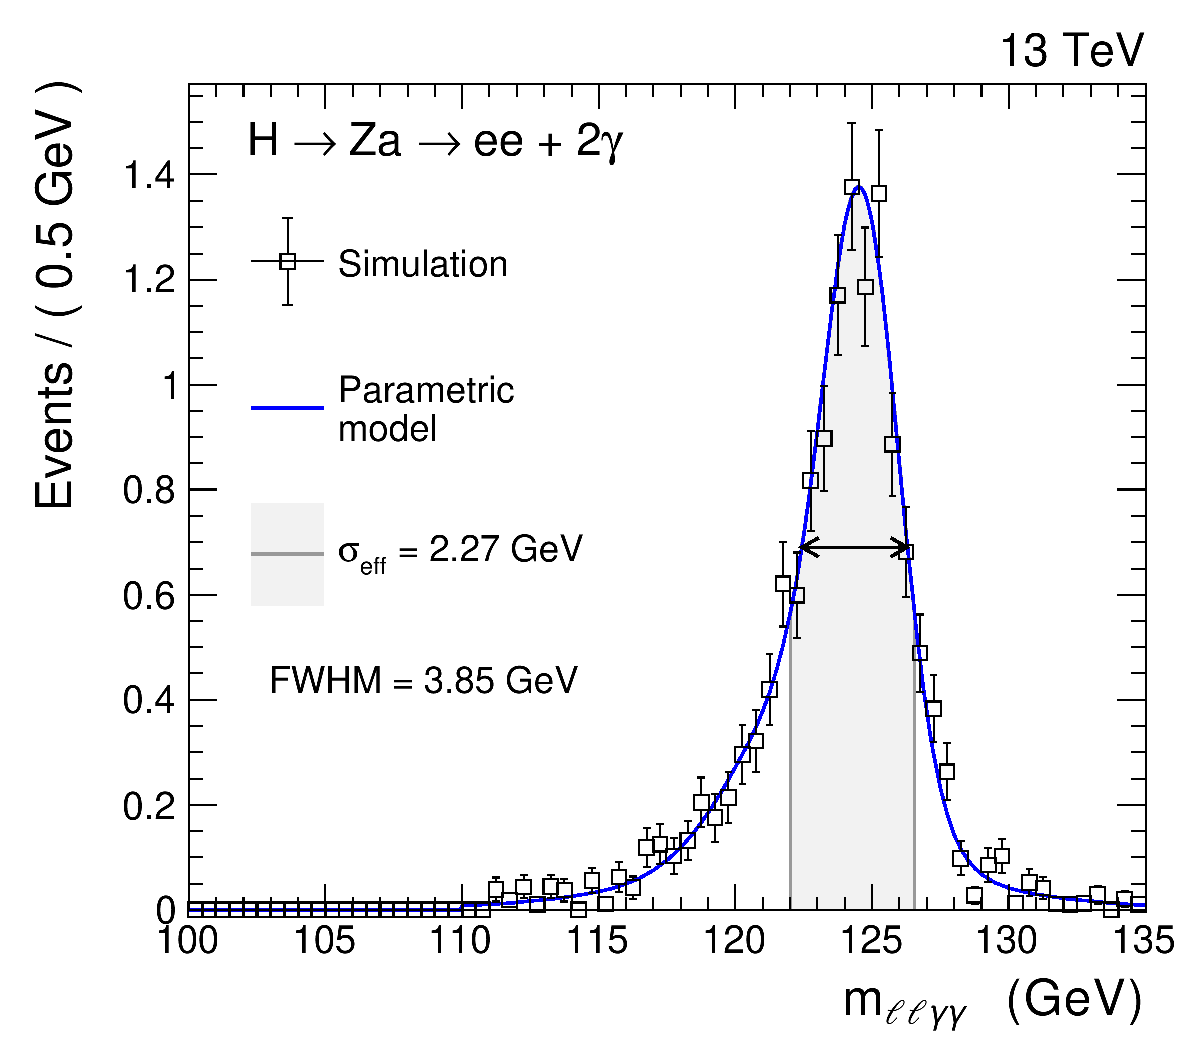
\includegraphics[width=0.5\textwidth,page=1]{figures/chapter04/sig_model/sigModel_M3_ele.pdf}
        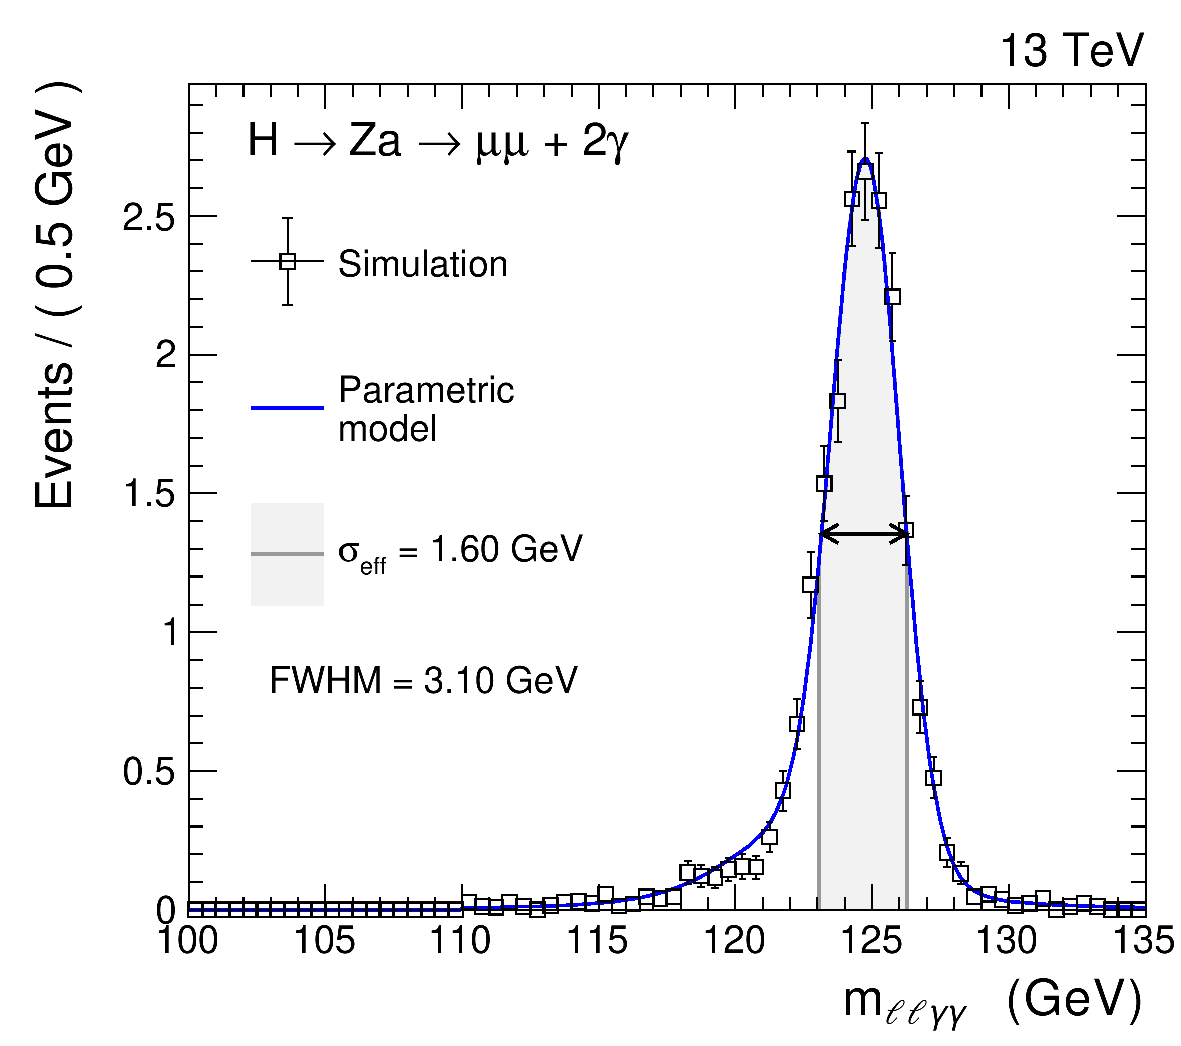
\includegraphics[width=0.5\textwidth,page=1]{figures/chapter04/sig_model/sigModel_M3_mu.pdf}
    \bicaption{\quad \centering 采用2016年post-VFP取数阶段的探测器设置,在电子(上图)和缪子(下图)道中拟合$\ma = 3~\si{GeV}$的信号事例样本的$\mllgg$分布。}{\quad \centering Fit of the $\mllgg$ distribution of signal events with $\ma = 3~\si{GeV}$ in the electron (top) and muon (bottom) channels with the detector settings of the 2016 post-VFP data-taking period.}
\end{center}
\end{figure}

\begin{figure}[htbp]
  \begin{center}
		\includegraphics[width=0.5\textwidth,page=2]{figures/chapter04/sig_model/sigModel_M3_ele.pdf}
        \includegraphics[width=0.5\textwidth,page=2]{figures/chapter04/sig_model/sigModel_M3_mu.pdf}
    \bicaption{\quad \centering 采用2016年pre-VFP取数阶段的探测器设置,在电子(上图)和缪子(下图)道中拟合$\ma = 3~\si{GeV}$的信号事例样本的$\mllgg$分布。}{\quad \centering Fit of the $\mllgg$ distribution of signal events with $\ma = 3~\si{GeV}$ in the electron (top) and muon (bottom) channels with the detector settings of the 2016 pre-VFP data-taking period.}
\end{center}
\end{figure}

\begin{figure}[htbp]
  \begin{center}
		\includegraphics[width=0.5\textwidth,page=3]{figures/chapter04/sig_model/sigModel_M3_ele.pdf}
        \includegraphics[width=0.5\textwidth,page=3]{figures/chapter04/sig_model/sigModel_M3_mu.pdf}
    \bicaption{\quad \centering 采用2017年取数阶段的探测器设置,在电子(上图)和缪子(下图)道中拟合$\ma = 3~\si{GeV}$的信号事例样本的$\mllgg$分布。}{\quad \centering Fit of the $\mllgg$ distribution of signal events with $\ma = 3~\si{GeV}$ in the electron (top) and muon (bottom) channels with the detector settings of the 2017 data-taking period.}
\end{center}
\end{figure}

\begin{figure}[htbp]
  \begin{center}
		\includegraphics[width=0.5\textwidth,page=4]{figures/chapter04/sig_model/sigModel_M3_ele.pdf}
        \includegraphics[width=0.5\textwidth,page=4]{figures/chapter04/sig_model/sigModel_M3_mu.pdf}
    \bicaption{\quad \centering 采用2018年取数阶段的探测器设置,在电子(上图)和缪子(下图)道中拟合$\ma = 3~\si{GeV}$的信号事例样本的$\mllgg$分布。}{\quad \centering Fit of the $\mllgg$ distribution of signal events with $\ma = 3~\si{GeV}$ in the electron (top) and muon (bottom) channels with the detector settings of the 2018 data-taking period.}
\end{center}
\end{figure}

\begin{figure}[htbp]
  \begin{center}
		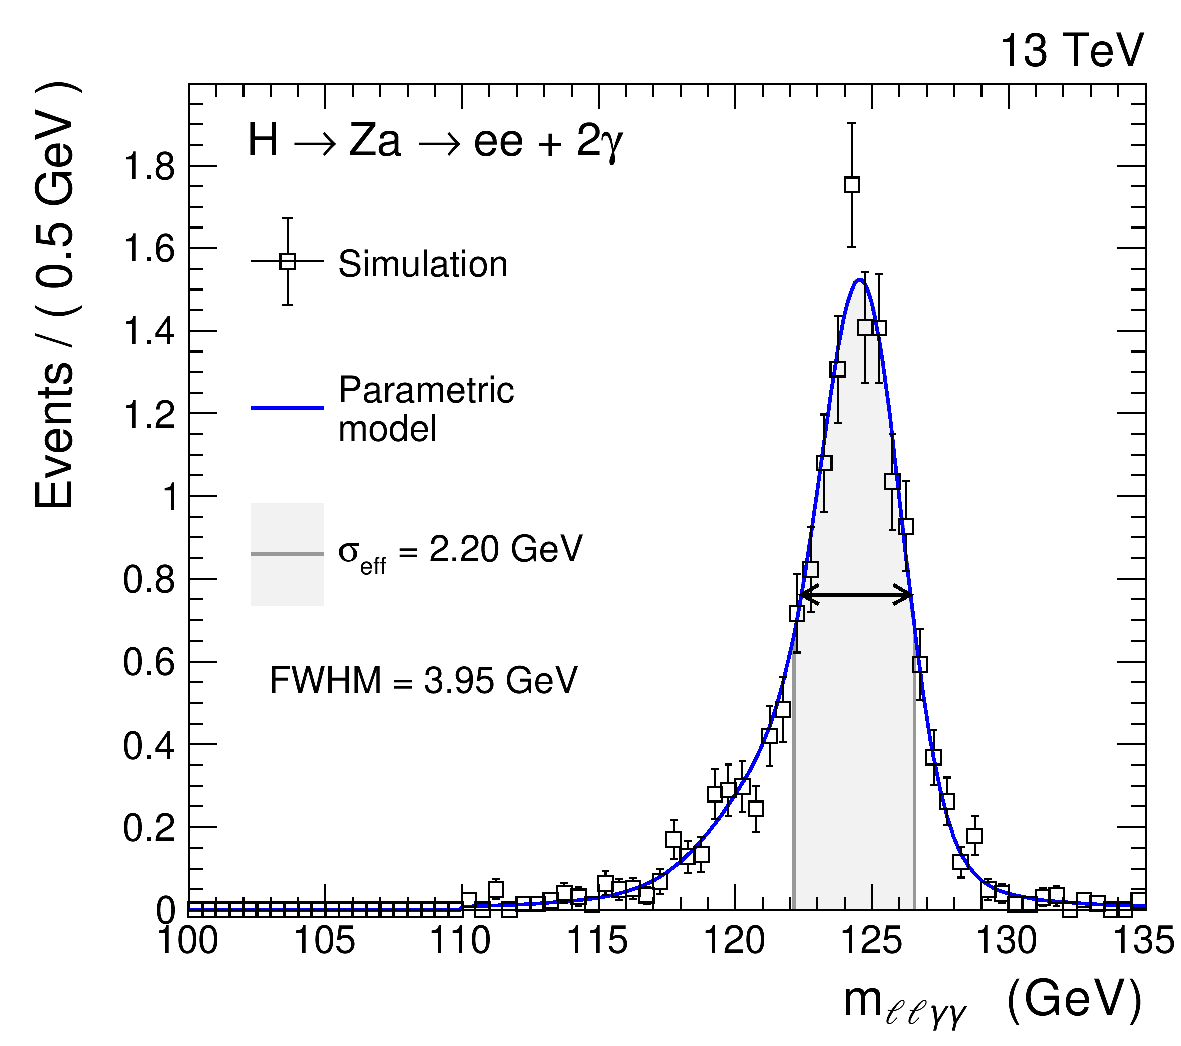
\includegraphics[width=0.5\textwidth,page=1]{figures/chapter04/sig_model/sigModel_M4_ele.pdf}
        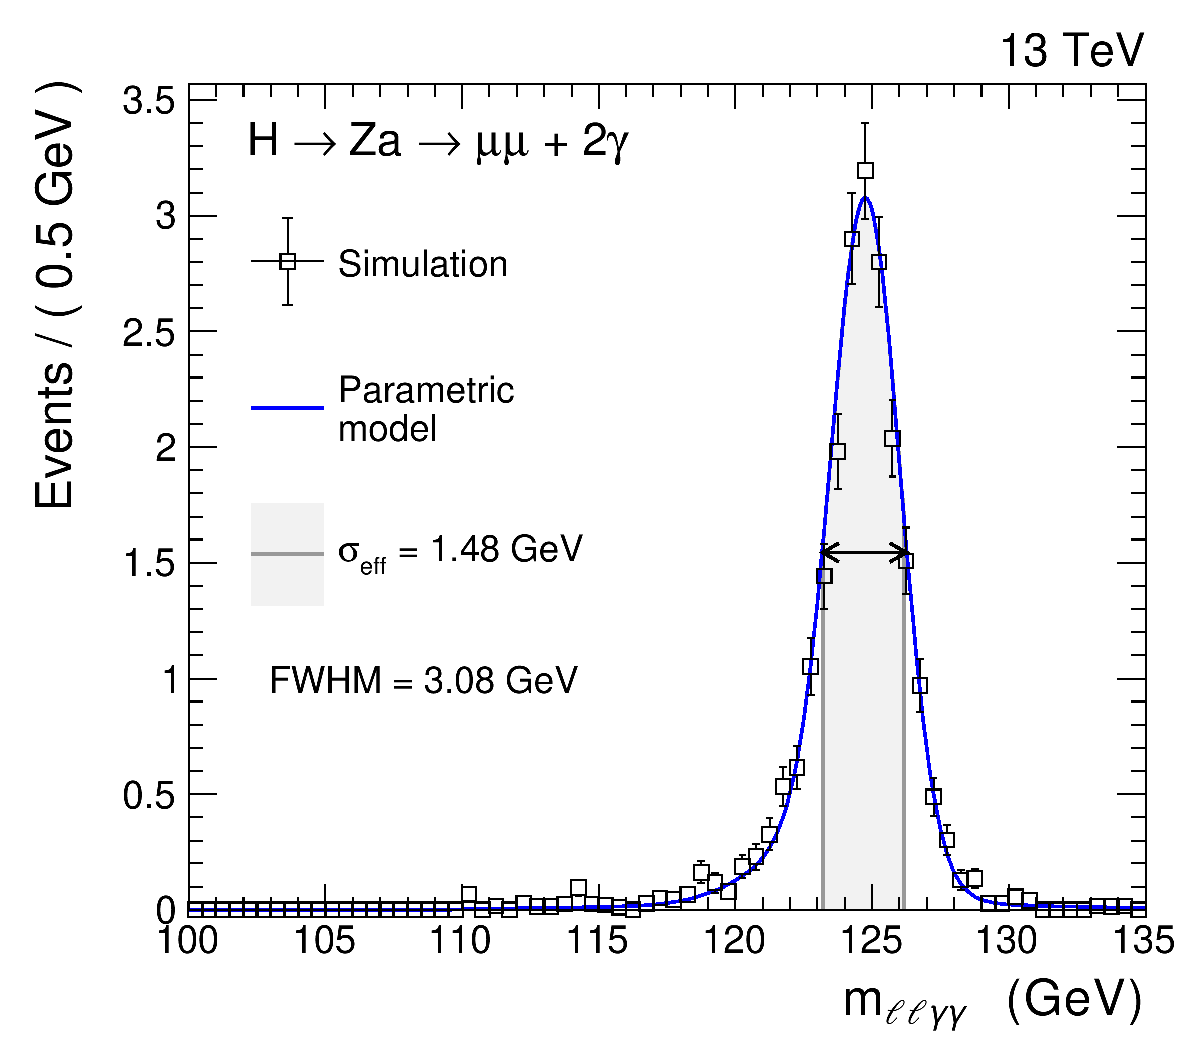
\includegraphics[width=0.5\textwidth,page=1]{figures/chapter04/sig_model/sigModel_M4_mu.pdf}
    \bicaption{\quad \centering 采用2016年post-VFP取数阶段的探测器设置,在电子(上图)和缪子(下图)道中拟合$\ma = 4~\si{GeV}$的信号事例样本的$\mllgg$分布。}{\quad \centering Fit of the $\mllgg$ distribution of signal events with $\ma = 4~\si{GeV}$ in the electron (top) and muon (bottom) channels with the detector settings of the 2016 post-VFP data-taking period.}
\end{center}
\end{figure}

\begin{figure}[htbp]
  \begin{center}
		\includegraphics[width=0.5\textwidth,page=2]{figures/chapter04/sig_model/sigModel_M4_ele.pdf}
        \includegraphics[width=0.5\textwidth,page=2]{figures/chapter04/sig_model/sigModel_M4_mu.pdf}
    \bicaption{\quad \centering 采用2016年pre-VFP取数阶段的探测器设置,在电子(上图)和缪子(下图)道中拟合$\ma = 4~\si{GeV}$的信号事例样本的$\mllgg$分布。}{\quad \centering Fit of the $\mllgg$ distribution of signal events with $\ma = 4~\si{GeV}$ in the electron (top) and muon (bottom) channels with the detector settings of the 2016 pre-VFP data-taking period.}
\end{center}
\end{figure}

\begin{figure}[htbp]
  \begin{center}
		\includegraphics[width=0.5\textwidth,page=3]{figures/chapter04/sig_model/sigModel_M4_ele.pdf}
        \includegraphics[width=0.5\textwidth,page=3]{figures/chapter04/sig_model/sigModel_M4_mu.pdf}
    \bicaption{\quad \centering 采用2017年取数阶段的探测器设置,在电子(上图)和缪子(下图)道中拟合$\ma = 4~\si{GeV}$的信号事例样本的$\mllgg$分布。}{\quad \centering Fit of the $\mllgg$ distribution of signal events with $\ma = 4~\si{GeV}$ in the electron (top) and muon (bottom) channels with the detector settings of the 2017 data-taking period.}
\end{center}
\end{figure}

\begin{figure}[htbp]
  \begin{center}
		\includegraphics[width=0.5\textwidth,page=4]{figures/chapter04/sig_model/sigModel_M4_ele.pdf}
        \includegraphics[width=0.5\textwidth,page=4]{figures/chapter04/sig_model/sigModel_M4_mu.pdf}
    \bicaption{\quad \centering 采用2018年取数阶段的探测器设置,在电子(上图)和缪子(下图)道中拟合$\ma = 4~\si{GeV}$的信号事例样本的$\mllgg$分布。}{\quad \centering Fit of the $\mllgg$ distribution of signal events with $\ma = 4~\si{GeV}$ in the electron (top) and muon (bottom) channels with the detector settings of the 2018 data-taking period.}
\end{center}
\end{figure}

\begin{figure}[htbp]
  \begin{center}
		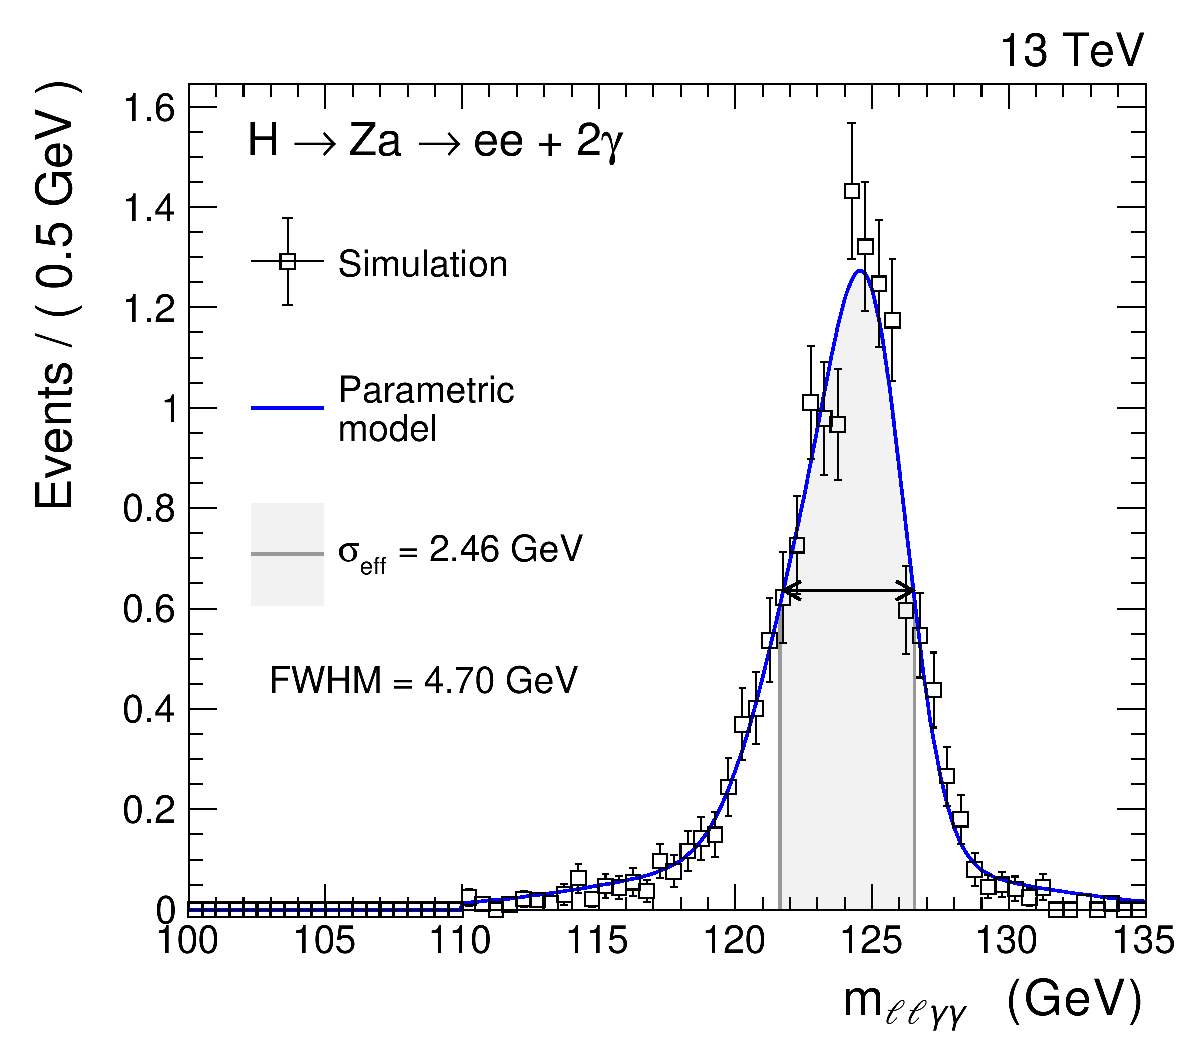
\includegraphics[width=0.5\textwidth,page=1]{figures/chapter04/sig_model/sigModel_M5_ele.pdf}
        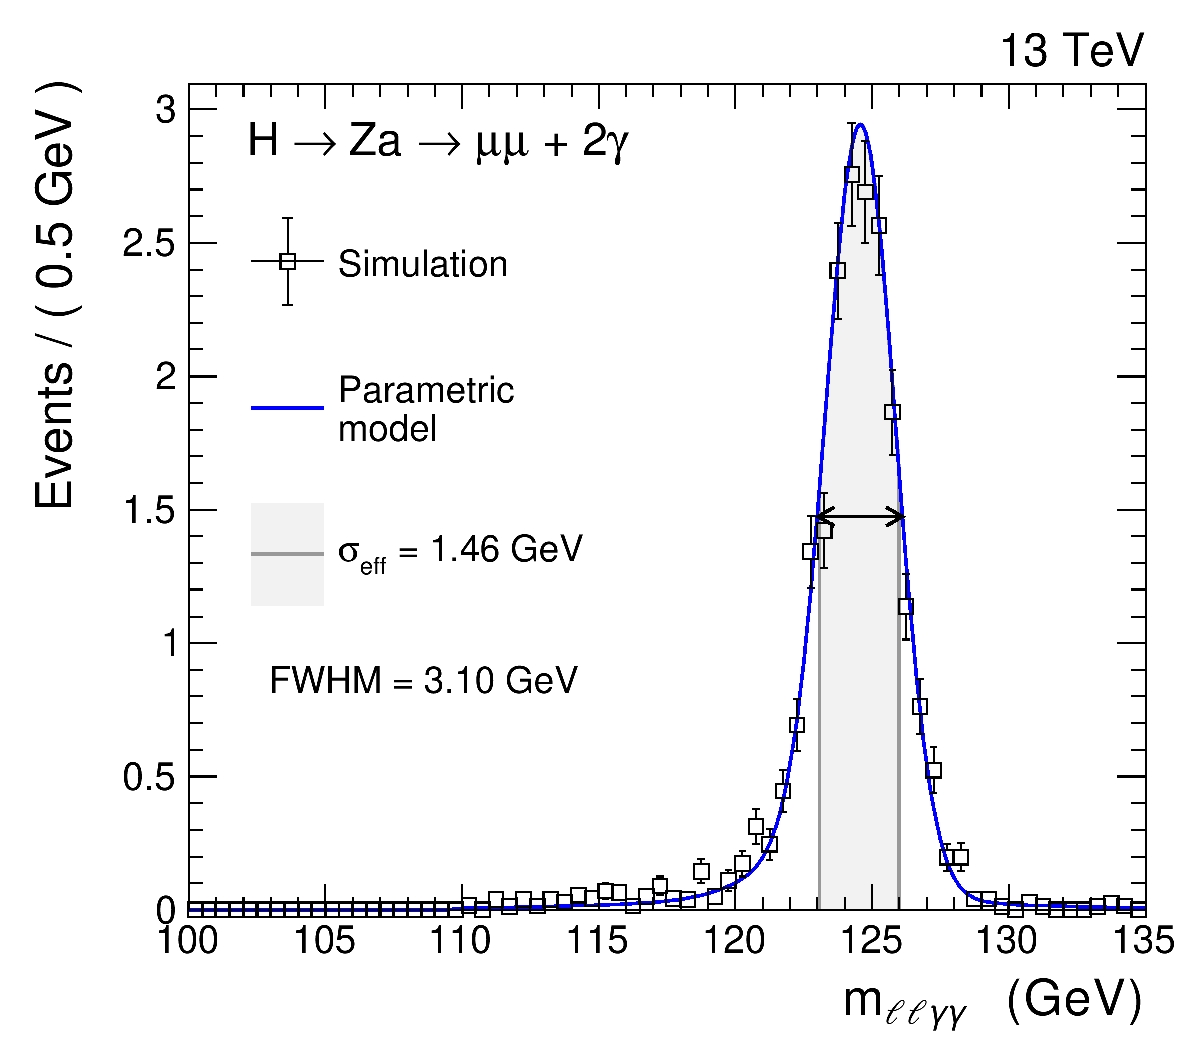
\includegraphics[width=0.5\textwidth,page=1]{figures/chapter04/sig_model/sigModel_M5_mu.pdf}
    \bicaption{\quad \centering 采用2016年post-VFP取数阶段的探测器设置,在电子(上图)和缪子(下图)道中拟合$\ma = 5~\si{GeV}$的信号事例样本的$\mllgg$分布。}{\quad \centering Fit of the $\mllgg$ distribution of signal events with $\ma = 5~\si{GeV}$ in the electron (top) and muon (bottom) channels with the detector settings of the 2016 post-VFP data-taking period.}
\end{center}
\end{figure}

\begin{figure}[htbp]
  \begin{center}
		\includegraphics[width=0.5\textwidth,page=2]{figures/chapter04/sig_model/sigModel_M5_ele.pdf}
        \includegraphics[width=0.5\textwidth,page=2]{figures/chapter04/sig_model/sigModel_M5_mu.pdf}
    \bicaption{\quad \centering 采用2016年pre-VFP取数阶段的探测器设置,在电子(上图)和缪子(下图)道中拟合$\ma = 5~\si{GeV}$的信号事例样本的$\mllgg$分布。}{\quad \centering Fit of the $\mllgg$ distribution of signal events with $\ma = 5~\si{GeV}$ in the electron (top) and muon (bottom) channels with the detector settings of the 2016 pre-VFP data-taking period.}
\end{center}
\end{figure}

\begin{figure}[htbp]
  \begin{center}
		\includegraphics[width=0.5\textwidth,page=3]{figures/chapter04/sig_model/sigModel_M5_ele.pdf}
        \includegraphics[width=0.5\textwidth,page=3]{figures/chapter04/sig_model/sigModel_M5_mu.pdf}
    \bicaption{\quad \centering 采用2017年取数阶段的探测器设置,在电子(上图)和缪子(下图)道中拟合$\ma = 5~\si{GeV}$的信号事例样本的$\mllgg$分布。}{\quad \centering Fit of the $\mllgg$ distribution of signal events with $\ma = 5~\si{GeV}$ in the electron (top) and muon (bottom) channels with the detector settings of the 2017 data-taking period.}
\end{center}
\end{figure}

\begin{figure}[htbp]
  \begin{center}
		\includegraphics[width=0.5\textwidth,page=4]{figures/chapter04/sig_model/sigModel_M5_ele.pdf}
        \includegraphics[width=0.5\textwidth,page=4]{figures/chapter04/sig_model/sigModel_M5_mu.pdf}
    \bicaption{\quad \centering 采用2018年取数阶段的探测器设置,在电子(上图)和缪子(下图)道中拟合$\ma = 5~\si{GeV}$的信号事例样本的$\mllgg$分布。}{\quad \centering Fit of the $\mllgg$ distribution of signal events with $\ma = 5~\si{GeV}$ in the electron (top) and muon (bottom) channels with the detector settings of the 2018 data-taking period.}
\end{center}
\end{figure}

\begin{figure}[htbp]
  \begin{center}
		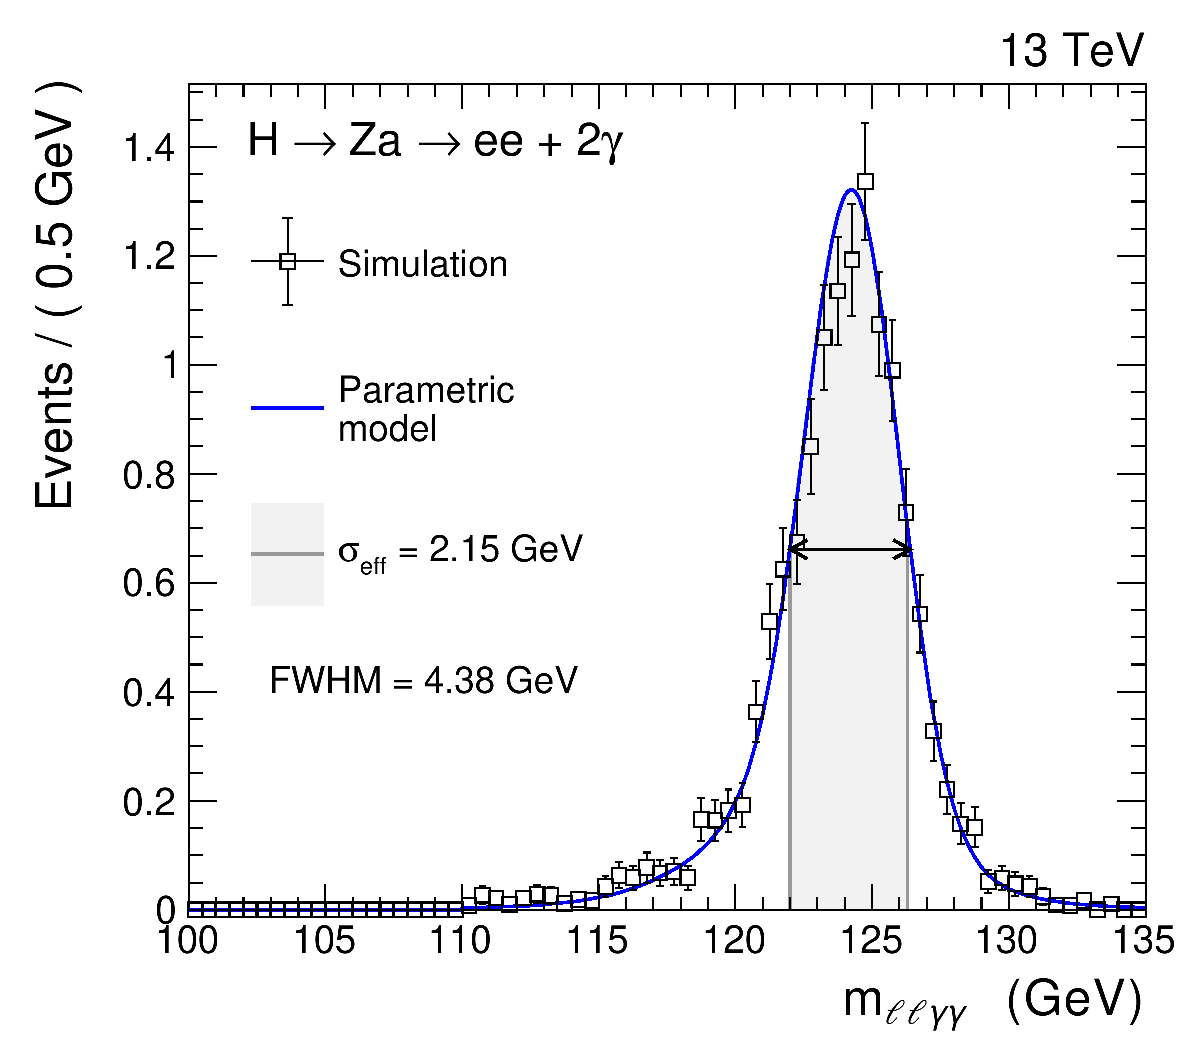
\includegraphics[width=0.5\textwidth,page=1]{figures/chapter04/sig_model/sigModel_M6_ele.pdf}
        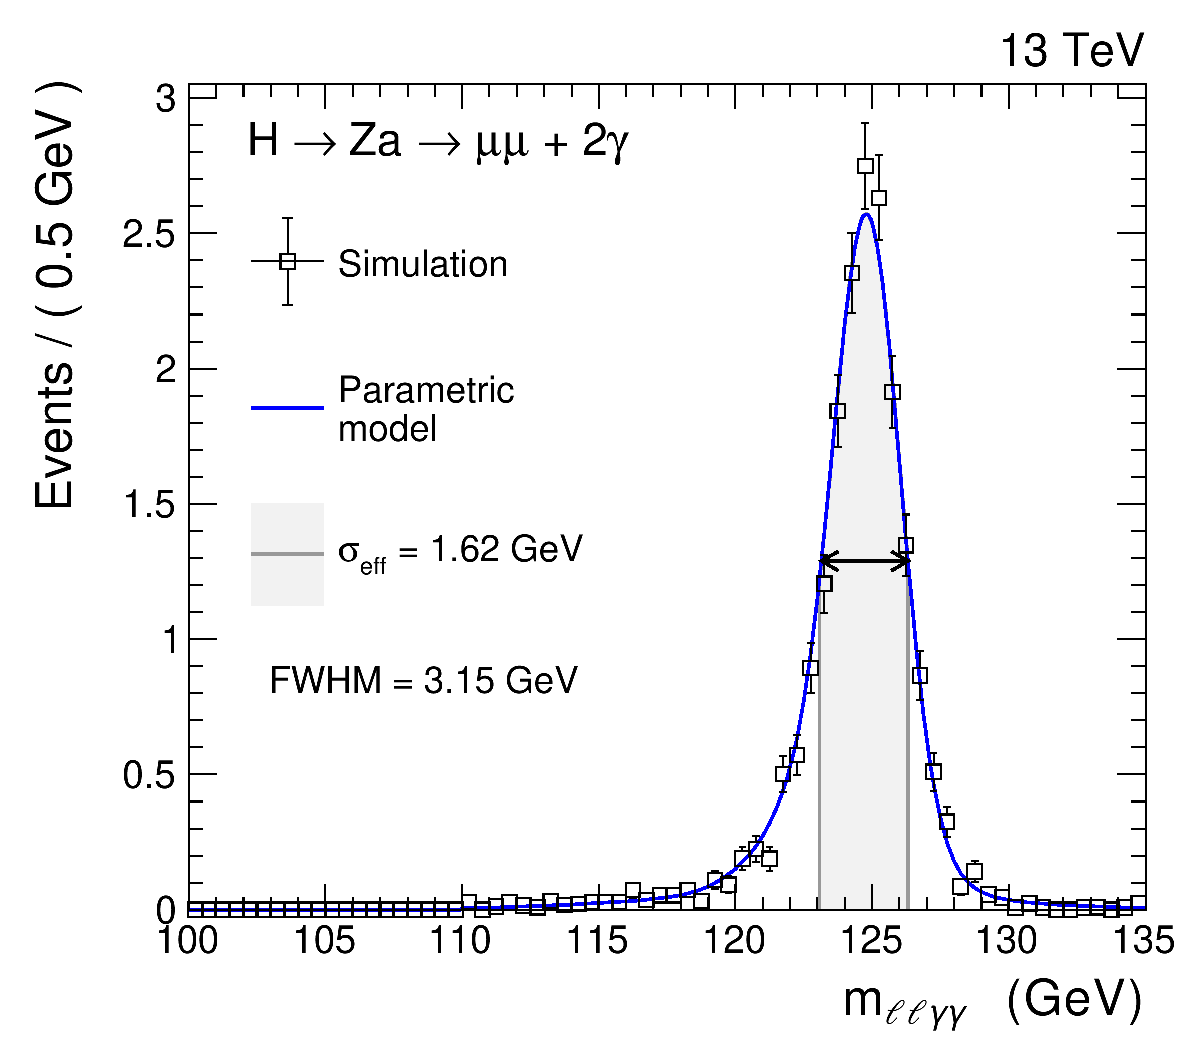
\includegraphics[width=0.5\textwidth,page=1]{figures/chapter04/sig_model/sigModel_M6_mu.pdf}
    \bicaption{\quad \centering 采用2016年post-VFP取数阶段的探测器设置,在电子(上图)和缪子(下图)道中拟合$\ma = 6~\si{GeV}$的信号事例样本的$\mllgg$分布。}{\quad \centering Fit of the $\mllgg$ distribution of signal events with $\ma = 6~\si{GeV}$ in the electron (top) and muon (bottom) channels with the detector settings of the 2016 post-VFP data-taking period.}
\end{center}
\end{figure}

\begin{figure}[htbp]
  \begin{center}
		\includegraphics[width=0.5\textwidth,page=2]{figures/chapter04/sig_model/sigModel_M6_ele.pdf}
        \includegraphics[width=0.5\textwidth,page=2]{figures/chapter04/sig_model/sigModel_M6_mu.pdf}
    \bicaption{\quad \centering 采用2016年pre-VFP取数阶段的探测器设置,在电子(上图)和缪子(下图)道中拟合$\ma = 6~\si{GeV}$的信号事例样本的$\mllgg$分布。}{\quad \centering Fit of the $\mllgg$ distribution of signal events with $\ma = 6~\si{GeV}$ in the electron (top) and muon (bottom) channels with the detector settings of the 2016 pre-VFP data-taking period.}
\end{center}
\end{figure}

\begin{figure}[htbp]
  \begin{center}
		\includegraphics[width=0.5\textwidth,page=3]{figures/chapter04/sig_model/sigModel_M6_ele.pdf}
        \includegraphics[width=0.5\textwidth,page=3]{figures/chapter04/sig_model/sigModel_M6_mu.pdf}
    \bicaption{\quad \centering 采用2017年取数阶段的探测器设置,在电子(上图)和缪子(下图)道中拟合$\ma = 6~\si{GeV}$的信号事例样本的$\mllgg$分布。}{\quad \centering Fit of the $\mllgg$ distribution of signal events with $\ma = 6~\si{GeV}$ in the electron (top) and muon (bottom) channels with the detector settings of the 2017 data-taking period.}
\end{center}
\end{figure}

\begin{figure}[htbp]
  \begin{center}
		\includegraphics[width=0.5\textwidth,page=4]{figures/chapter04/sig_model/sigModel_M6_ele.pdf}
        \includegraphics[width=0.5\textwidth,page=4]{figures/chapter04/sig_model/sigModel_M6_mu.pdf}
    \bicaption{\quad \centering 采用2018年取数阶段的探测器设置,在电子(上图)和缪子(下图)道中拟合$\ma = 6~\si{GeV}$的信号事例样本的$\mllgg$分布。}{\quad \centering Fit of the $\mllgg$ distribution of signal events with $\ma = 6~\si{GeV}$ in the electron (top) and muon (bottom) channels with the detector settings of the 2018 data-taking period.}
\end{center}
\end{figure}


\begin{figure}[htbp]
  \begin{center}
		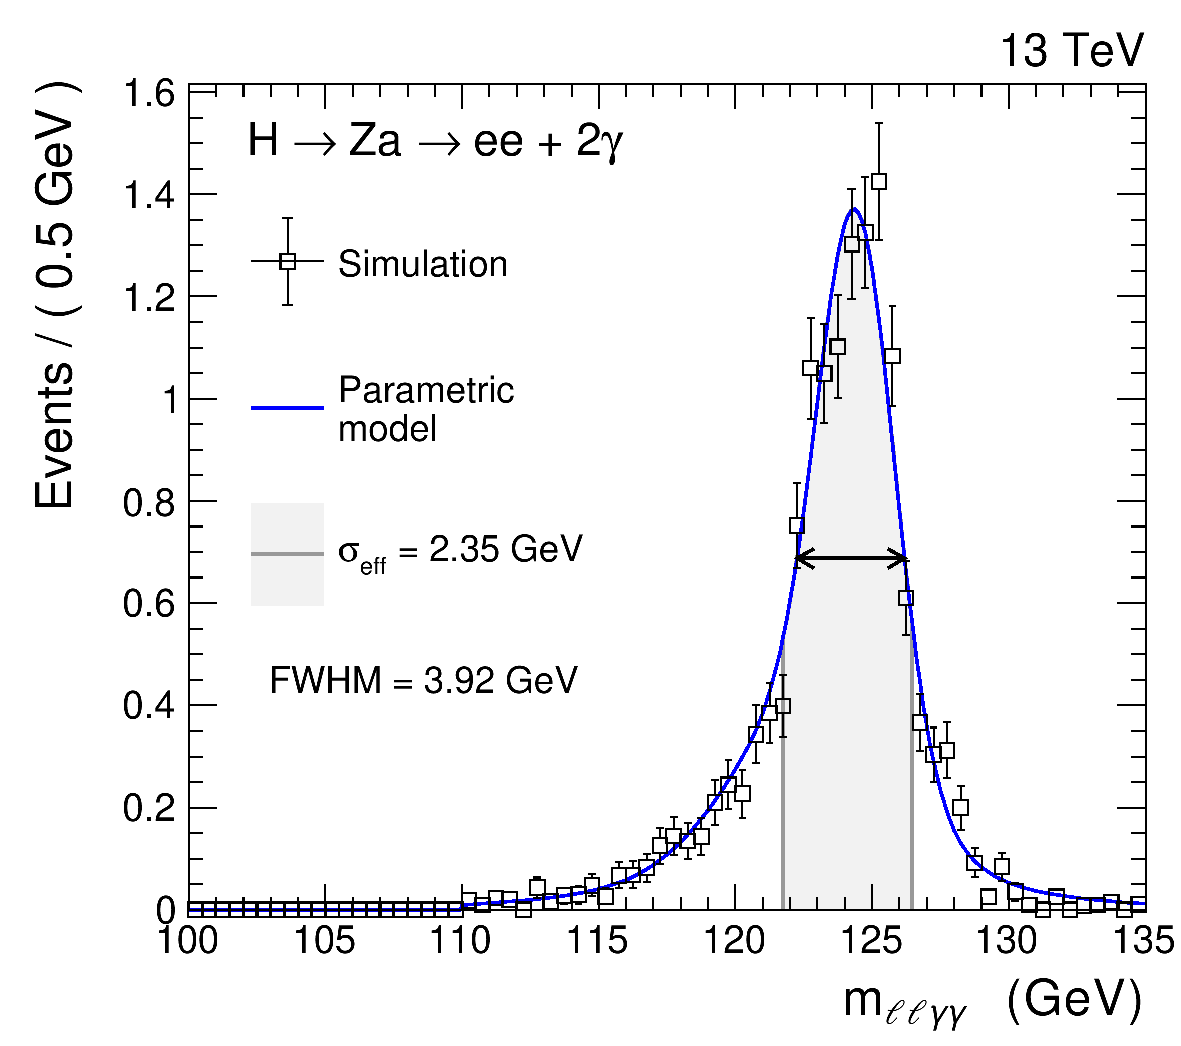
\includegraphics[width=0.5\textwidth,page=1]{figures/chapter04/sig_model/sigModel_M7_ele.pdf}
        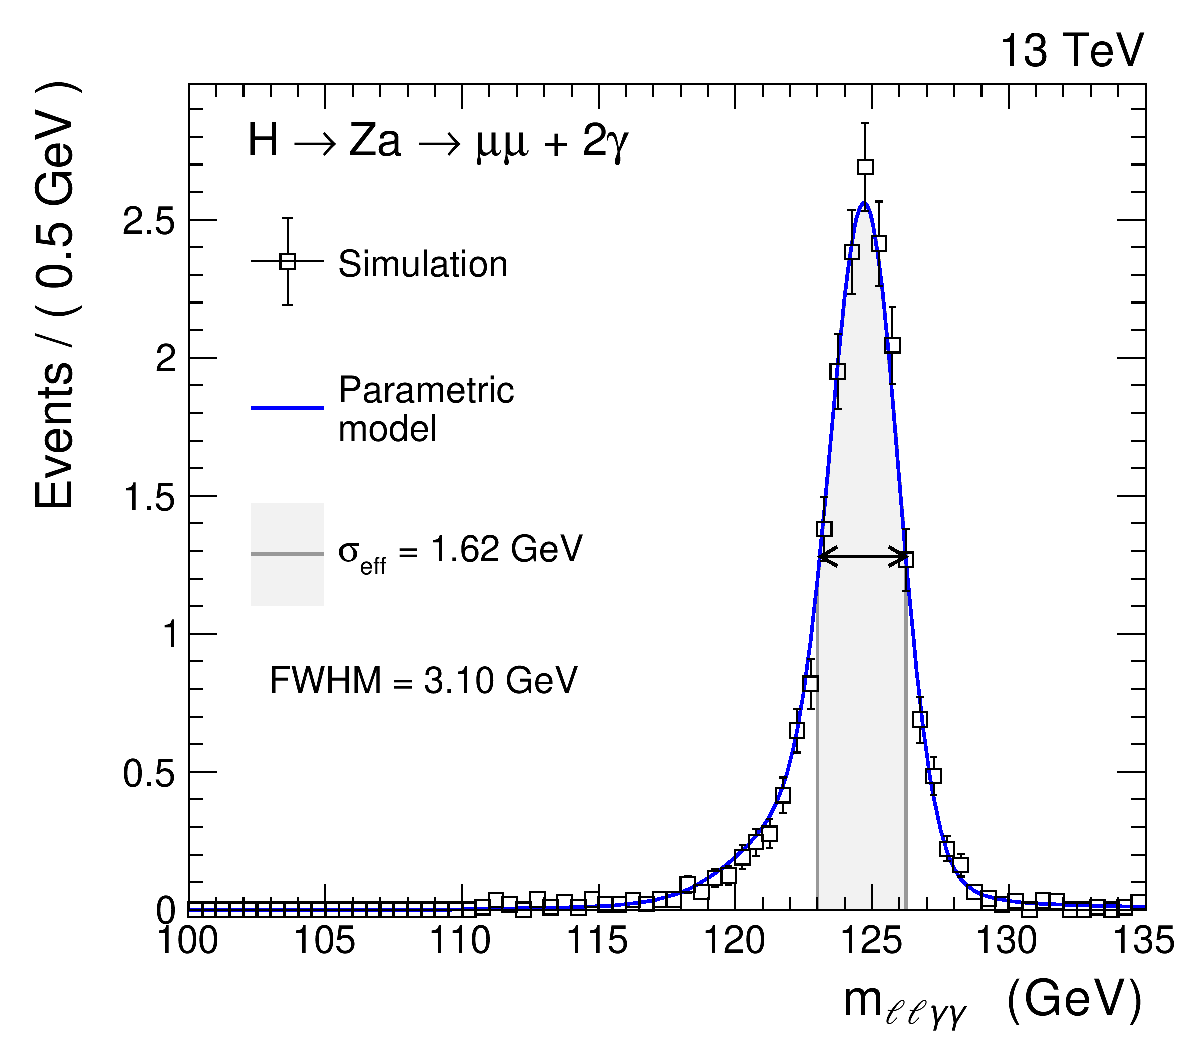
\includegraphics[width=0.5\textwidth,page=1]{figures/chapter04/sig_model/sigModel_M7_mu.pdf}
    \bicaption{\quad \centering 采用2016年post-VFP取数阶段的探测器设置,在电子(上图)和缪子(下图)道中拟合$\ma = 7~\si{GeV}$的信号事例样本的$\mllgg$分布。}{\quad \centering Fit of the $\mllgg$ distribution of signal events with $\ma = 7~\si{GeV}$ in the electron (top) and muon (bottom) channels with the detector settings of the 2016 post-VFP data-taking period.}
\end{center}
\end{figure}

\begin{figure}[htbp]
  \begin{center}
		\includegraphics[width=0.5\textwidth,page=2]{figures/chapter04/sig_model/sigModel_M7_ele.pdf}
        \includegraphics[width=0.5\textwidth,page=2]{figures/chapter04/sig_model/sigModel_M7_mu.pdf}
    \bicaption{\quad \centering 采用2016年pre-VFP取数阶段的探测器设置,在电子(上图)和缪子(下图)道中拟合$\ma = 7~\si{GeV}$的信号事例样本的$\mllgg$分布。}{\quad \centering Fit of the $\mllgg$ distribution of signal events with $\ma = 7~\si{GeV}$ in the electron (top) and muon (bottom) channels with the detector settings of the 2016 pre-VFP data-taking period.}
\end{center}
\end{figure}

\begin{figure}[htbp]
  \begin{center}
		\includegraphics[width=0.5\textwidth,page=3]{figures/chapter04/sig_model/sigModel_M7_ele.pdf}
        \includegraphics[width=0.5\textwidth,page=3]{figures/chapter04/sig_model/sigModel_M7_mu.pdf}
    \bicaption{\quad \centering 采用2017年取数阶段的探测器设置,在电子(上图)和缪子(下图)道中拟合$\ma = 7~\si{GeV}$的信号事例样本的$\mllgg$分布。}{\quad \centering Fit of the $\mllgg$ distribution of signal events with $\ma = 7~\si{GeV}$ in the electron (top) and muon (bottom) channels with the detector settings of the 2017 data-taking period.}
\end{center}
\end{figure}

\begin{figure}[htbp]
  \begin{center}
		\includegraphics[width=0.5\textwidth,page=4]{figures/chapter04/sig_model/sigModel_M7_ele.pdf}
        \includegraphics[width=0.5\textwidth,page=4]{figures/chapter04/sig_model/sigModel_M7_mu.pdf}
    \bicaption{\quad \centering 采用2018年取数阶段的探测器设置,在电子(上图)和缪子(下图)道中拟合$\ma = 7~\si{GeV}$的信号事例样本的$\mllgg$分布。}{\quad \centering Fit of the $\mllgg$ distribution of signal events with $\ma = 7~\si{GeV}$ in the electron (top) and muon (bottom) channels with the detector settings of the 2018 data-taking period.}
\end{center}
\end{figure}

\begin{figure}[htbp]
  \begin{center}
		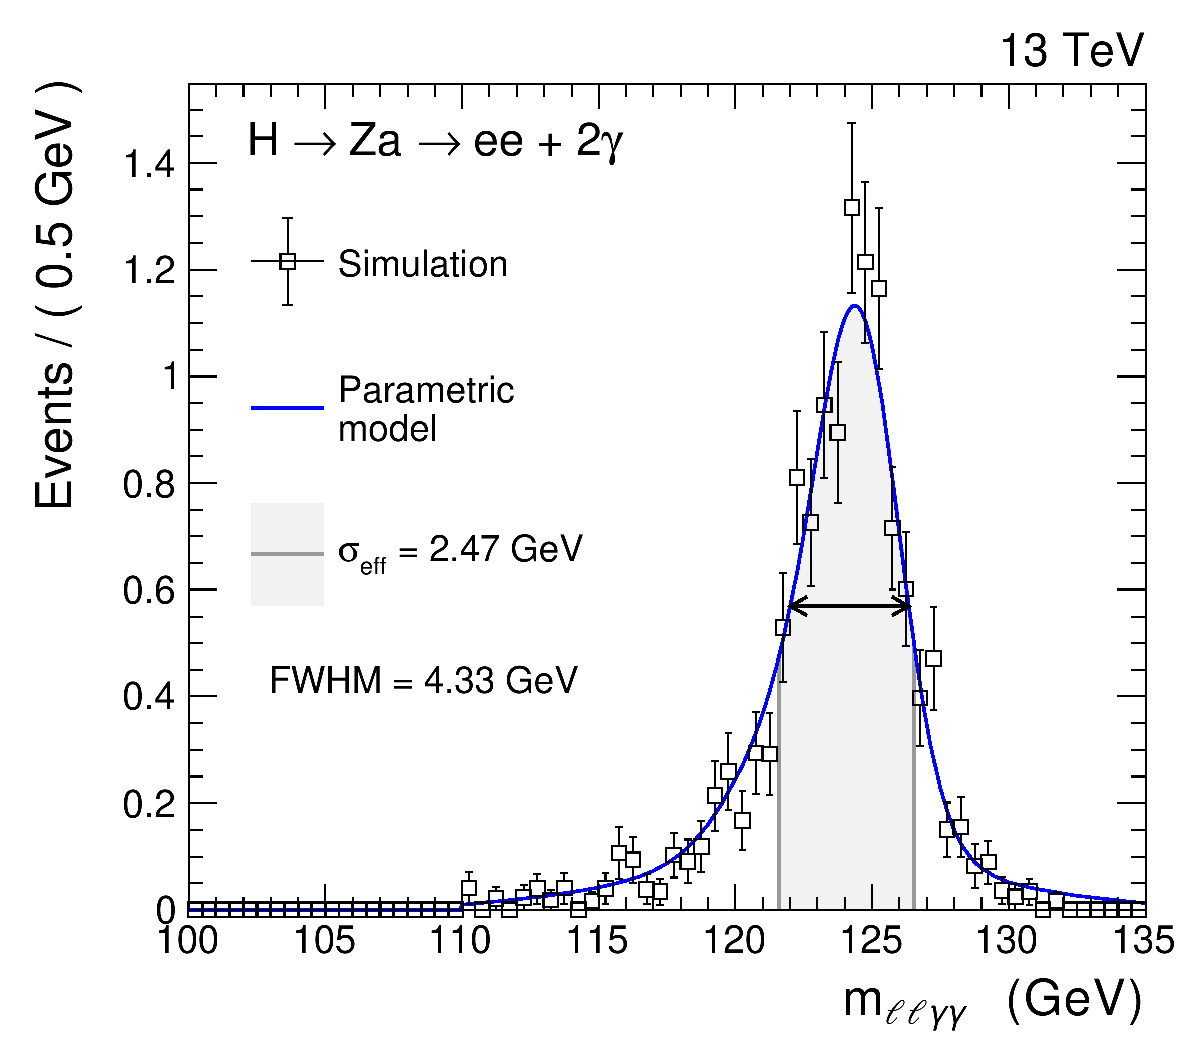
\includegraphics[width=0.5\textwidth,page=1]{figures/chapter04/sig_model/sigModel_M8_ele.pdf}
        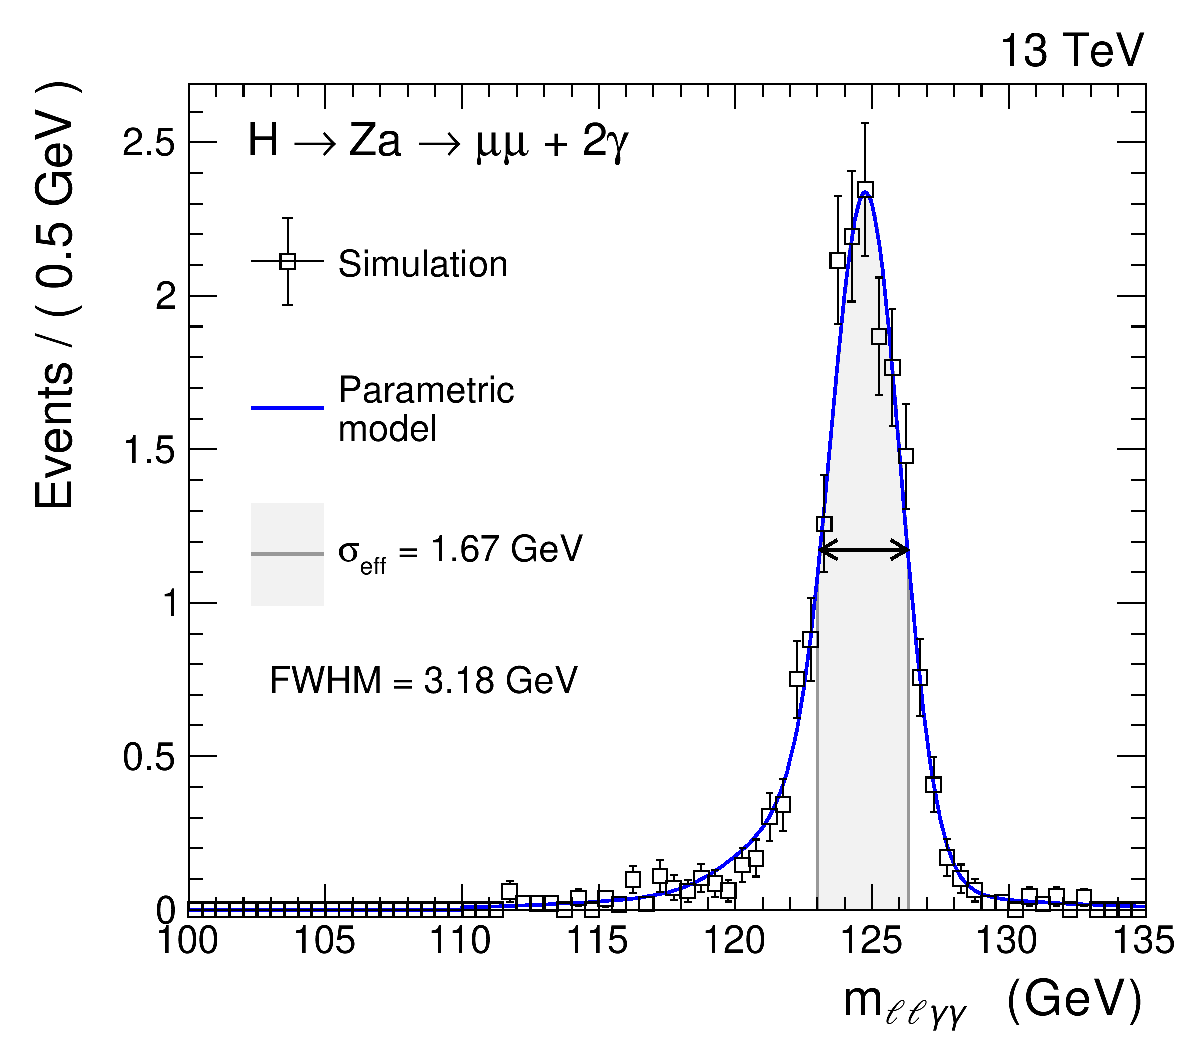
\includegraphics[width=0.5\textwidth,page=1]{figures/chapter04/sig_model/sigModel_M8_mu.pdf}
    \bicaption{\quad \centering 采用2016年post-VFP取数阶段的探测器设置,在电子(上图)和缪子(下图)道中拟合$\ma = 8~\si{GeV}$的信号事例样本的$\mllgg$分布。}{\quad \centering Fit of the $\mllgg$ distribution of signal events with $\ma = 8~\si{GeV}$ in the electron (top) and muon (bottom) channels with the detector settings of the 2016 post-VFP data-taking period.}
\end{center}
\end{figure}

\begin{figure}[htbp]
  \begin{center}
		\includegraphics[width=0.5\textwidth,page=2]{figures/chapter04/sig_model/sigModel_M8_ele.pdf}
        \includegraphics[width=0.5\textwidth,page=2]{figures/chapter04/sig_model/sigModel_M8_mu.pdf}
    \bicaption{\quad \centering 采用2016年pre-VFP取数阶段的探测器设置,在电子(上图)和缪子(下图)道中拟合$\ma = 8~\si{GeV}$的信号事例样本的$\mllgg$分布。}{\quad \centering Fit of the $\mllgg$ distribution of signal events with $\ma = 8~\si{GeV}$ in the electron (top) and muon (bottom) channels with the detector settings of the 2016 pre-VFP data-taking period.}
\end{center}
\end{figure}

\begin{figure}[htbp]
  \begin{center}
		\includegraphics[width=0.5\textwidth,page=3]{figures/chapter04/sig_model/sigModel_M8_ele.pdf}
        \includegraphics[width=0.5\textwidth,page=3]{figures/chapter04/sig_model/sigModel_M8_mu.pdf}
    \bicaption{\quad \centering 采用2017年取数阶段的探测器设置,在电子(上图)和缪子(下图)道中拟合$\ma = 8~\si{GeV}$的信号事例样本的$\mllgg$分布。}{\quad \centering Fit of the $\mllgg$ distribution of signal events with $\ma = 8~\si{GeV}$ in the electron (top) and muon (bottom) channels with the detector settings of the 2017 data-taking period.}
\end{center}
\end{figure}

\begin{figure}[htbp]
  \begin{center}
		\includegraphics[width=0.5\textwidth,page=4]{figures/chapter04/sig_model/sigModel_M8_ele.pdf}
        \includegraphics[width=0.5\textwidth,page=4]{figures/chapter04/sig_model/sigModel_M8_mu.pdf}
    \bicaption{\quad \centering 采用2018年取数阶段的探测器设置,在电子(上图)和缪子(下图)道中拟合$\ma = 8~\si{GeV}$的信号事例样本的$\mllgg$分布。}{\quad \centering Fit of the $\mllgg$ distribution of signal events with $\ma = 8~\si{GeV}$ in the electron (top) and muon (bottom) channels with the detector settings of the 2018 data-taking period.}
\end{center}
\end{figure}

\begin{figure}[htbp]
  \begin{center}
		\includegraphics[width=0.5\textwidth,page=1]{figures/chapter04/sig_model/sigModel_M9_ele.pdf}
        \includegraphics[width=0.5\textwidth,page=1]{figures/chapter04/sig_model/sigModel_M9_mu.pdf}
    \bicaption{\quad \centering 采用2016年post-VFP取数阶段的探测器设置,在电子(上图)和缪子(下图)道中拟合$\ma = 9~\si{GeV}$的信号事例样本的$\mllgg$分布。}{\quad \centering Fit of the $\mllgg$ distribution of signal events with $\ma = 9~\si{GeV}$ in the electron (top) and muon (bottom) channels with the detector settings of the 2016 post-VFP data-taking period.}
\end{center}
\end{figure}

\begin{figure}[htbp]
  \begin{center}
		\includegraphics[width=0.5\textwidth,page=2]{figures/chapter04/sig_model/sigModel_M9_ele.pdf}
        \includegraphics[width=0.5\textwidth,page=2]{figures/chapter04/sig_model/sigModel_M9_mu.pdf}
    \bicaption{\quad \centering 采用2016年pre-VFP取数阶段的探测器设置,在电子(上图)和缪子(下图)道中拟合$\ma = 9~\si{GeV}$的信号事例样本的$\mllgg$分布。}{\quad \centering Fit of the $\mllgg$ distribution of signal events with $\ma = 9~\si{GeV}$ in the electron (top) and muon (bottom) channels with the detector settings of the 2016 pre-VFP data-taking period.}
\end{center}
\end{figure}

\begin{figure}[htbp]
  \begin{center}
		\includegraphics[width=0.5\textwidth,page=3]{figures/chapter04/sig_model/sigModel_M9_ele.pdf}
        \includegraphics[width=0.5\textwidth,page=3]{figures/chapter04/sig_model/sigModel_M9_mu.pdf}
    \bicaption{\quad \centering 采用2017年取数阶段的探测器设置,在电子(上图)和缪子(下图)道中拟合$\ma = 9~\si{GeV}$的信号事例样本的$\mllgg$分布。}{\quad \centering Fit of the $\mllgg$ distribution of signal events with $\ma = 9~\si{GeV}$ in the electron (top) and muon (bottom) channels with the detector settings of the 2017 data-taking period.}
\end{center}
\end{figure}

\begin{figure}[htbp]
  \begin{center}
		\includegraphics[width=0.5\textwidth,page=4]{figures/chapter04/sig_model/sigModel_M9_ele.pdf}
        \includegraphics[width=0.5\textwidth,page=4]{figures/chapter04/sig_model/sigModel_M9_mu.pdf}
    \bicaption{\quad \centering 采用2018年取数阶段的探测器设置,在电子(上图)和缪子(下图)道中拟合$\ma = 9~\si{GeV}$的信号事例样本的$\mllgg$分布。}{\quad \centering Fit of the $\mllgg$ distribution of signal events with $\ma = 9~\si{GeV}$ in the electron (top) and muon (bottom) channels with the detector settings of the 2018 data-taking period.}
\end{center}
\end{figure}

\begin{figure}[htbp]
  \begin{center}
		\includegraphics[width=0.5\textwidth,page=1]{figures/chapter04/sig_model/sigModel_M10_ele.pdf}
        \includegraphics[width=0.5\textwidth,page=1]{figures/chapter04/sig_model/sigModel_M10_mu.pdf}
    \bicaption{\quad \centering 采用2016年post-VFP取数阶段的探测器设置,在电子(上图)和缪子(下图)道中拟合$\ma = 10~\si{GeV}$的信号事例样本的$\mllgg$分布。}{\quad \centering Fit of the $\mllgg$ distribution of signal events with $\ma = 10~\si{GeV}$ in the electron (top) and muon (bottom) channels with the detector settings of the 2016 post-VFP data-taking period.}
\end{center}
\end{figure}

\begin{figure}[htbp]
  \begin{center}
		\includegraphics[width=0.5\textwidth,page=2]{figures/chapter04/sig_model/sigModel_M10_ele.pdf}
        \includegraphics[width=0.5\textwidth,page=2]{figures/chapter04/sig_model/sigModel_M10_mu.pdf}
    \bicaption{\quad \centering 采用2016年pre-VFP取数阶段的探测器设置,在电子(上图)和缪子(下图)道中拟合$\ma = 10~\si{GeV}$的信号事例样本的$\mllgg$分布。}{\quad \centering Fit of the $\mllgg$ distribution of signal events with $\ma = 10~\si{GeV}$ in the electron (top) and muon (bottom) channels with the detector settings of the 2016 pre-VFP data-taking period.}
\end{center}
\end{figure}

\begin{figure}[htbp]
  \begin{center}
		\includegraphics[width=0.5\textwidth,page=3]{figures/chapter04/sig_model/sigModel_M10_ele.pdf}
        \includegraphics[width=0.5\textwidth,page=3]{figures/chapter04/sig_model/sigModel_M10_mu.pdf}
    \bicaption{\quad \centering 采用2017年取数阶段的探测器设置,在电子(上图)和缪子(下图)道中拟合$\ma = 10~\si{GeV}$的信号事例样本的$\mllgg$分布。}{\quad \centering Fit of the $\mllgg$ distribution of signal events with $\ma = 10~\si{GeV}$ in the electron (top) and muon (bottom) channels with the detector settings of the 2017 data-taking period.}
\end{center}
\end{figure}

\begin{figure}[htbp]
  \begin{center}
		\includegraphics[width=0.5\textwidth,page=4]{figures/chapter04/sig_model/sigModel_M10_ele.pdf}
        \includegraphics[width=0.5\textwidth,page=4]{figures/chapter04/sig_model/sigModel_M10_mu.pdf}
    \bicaption{\quad \centering 采用2018年取数阶段的探测器设置,在电子(上图)和缪子(下图)道中拟合$\ma = 10~\si{GeV}$的信号事例样本的$\mllgg$分布。}{\quad \centering Fit of the $\mllgg$ distribution of signal events with $\ma = 10~\si{GeV}$ in the electron (top) and muon (bottom) channels with the detector settings of the 2018 data-taking period.}
\end{center}
\end{figure}

\begin{figure}[htbp]
  \begin{center}
		\includegraphics[width=0.5\textwidth,page=1]{figures/chapter04/sig_model/sigModel_M15_ele.pdf}
        \includegraphics[width=0.5\textwidth,page=1]{figures/chapter04/sig_model/sigModel_M15_mu.pdf}
    \bicaption{\quad \centering 采用2016年post-VFP取数阶段的探测器设置,在电子(上图)和缪子(下图)道中拟合$\ma = 2~\si{GeV}$的信号事例样本的$\mllgg$分布。}{\quad \centering Fit of the $\mllgg$ distribution of signal events with $\ma = 15~\si{GeV}$ in the electron (top) and muon (bottom) channels with the detector settings of the 2016 post-VFP data-taking period.}
\end{center}
\end{figure}

\begin{figure}[htbp]
  \begin{center}
		\includegraphics[width=0.5\textwidth,page=2]{figures/chapter04/sig_model/sigModel_M15_ele.pdf}
        \includegraphics[width=0.5\textwidth,page=2]{figures/chapter04/sig_model/sigModel_M15_mu.pdf}
    \bicaption{\quad \centering 采用2016年pre-VFP取数阶段的探测器设置,在电子(上图)和缪子(下图)道中拟合$\ma = 15~\si{GeV}$的信号事例样本的$\mllgg$分布。}{\quad \centering Fit of the $\mllgg$ distribution of signal events with $\ma = 15~\si{GeV}$ in the electron (top) and muon (bottom) channels with the detector settings of the 2016 pre-VFP data-taking period.}
\end{center}
\end{figure}

\begin{figure}[htbp]
  \begin{center}
		\includegraphics[width=0.5\textwidth,page=3]{figures/chapter04/sig_model/sigModel_M15_ele.pdf}
        \includegraphics[width=0.5\textwidth,page=3]{figures/chapter04/sig_model/sigModel_M15_mu.pdf}
    \bicaption{\quad \centering 采用2017年取数阶段的探测器设置,在电子(上图)和缪子(下图)道中拟合$\ma = 15~\si{GeV}$的信号事例样本的$\mllgg$分布。}{\quad \centering Fit of the $\mllgg$ distribution of signal events with $\ma = 15~\si{GeV}$ in the electron (top) and muon (bottom) channels with the detector settings of the 2017 data-taking period.}
\end{center}
\end{figure}

\begin{figure}[htbp]
  \begin{center}
		\includegraphics[width=0.5\textwidth,page=4]{figures/chapter04/sig_model/sigModel_M15_ele.pdf}
        \includegraphics[width=0.5\textwidth,page=4]{figures/chapter04/sig_model/sigModel_M15_mu.pdf}
    \bicaption{\quad \centering 采用2018年取数阶段的探测器设置,在电子(上图)和缪子(下图)道中拟合$\ma = 15~\si{GeV}$的信号事例样本的$\mllgg$分布。}{\quad \centering Fit of the $\mllgg$ distribution of signal events with $\ma = 15~\si{GeV}$ in the electron (top) and muon (bottom) channels with the detector settings of the 2018 data-taking period.}
\end{center}
\end{figure}


\begin{figure}[htbp]
  \begin{center}
		\includegraphics[width=0.5\textwidth,page=1]{figures/chapter04/sig_model/sigModel_M20_ele.pdf}
        \includegraphics[width=0.5\textwidth,page=1]{figures/chapter04/sig_model/sigModel_M20_mu.pdf}
    \bicaption{\quad \centering 采用2016年post-VFP取数阶段的探测器设置,在电子(上图)和缪子(下图)道中拟合$\ma = 20~\si{GeV}$的信号事例样本的$\mllgg$分布。}{\quad \centering Fit of the $\mllgg$ distribution of signal events with $\ma = 20~\si{GeV}$ in the electron (top) and muon (bottom) channels with the detector settings of the 2016 post-VFP data-taking period.}
\end{center}
\end{figure}

\begin{figure}[htbp]
  \begin{center}
		\includegraphics[width=0.5\textwidth,page=2]{figures/chapter04/sig_model/sigModel_M20_ele.pdf}
        \includegraphics[width=0.5\textwidth,page=2]{figures/chapter04/sig_model/sigModel_M20_mu.pdf}
    \bicaption{\quad \centering 采用2016年pre-VFP取数阶段的探测器设置,在电子(上图)和缪子(下图)道中拟合$\ma = 20~\si{GeV}$的信号事例样本的$\mllgg$分布。}{\quad \centering Fit of the $\mllgg$ distribution of signal events with $\ma = 20~\si{GeV}$ in the electron (top) and muon (bottom) channels with the detector settings of the 2016 pre-VFP data-taking period.}
\end{center}
\end{figure}

\begin{figure}[htbp]
  \begin{center}
		\includegraphics[width=0.5\textwidth,page=3]{figures/chapter04/sig_model/sigModel_M20_ele.pdf}
        \includegraphics[width=0.5\textwidth,page=3]{figures/chapter04/sig_model/sigModel_M20_mu.pdf}
    \bicaption{\quad \centering 采用2017年取数阶段的探测器设置,在电子(上图)和缪子(下图)道中拟合$\ma = 20~\si{GeV}$的信号事例样本的$\mllgg$分布。}{\quad \centering Fit of the $\mllgg$ distribution of signal events with $\ma = 20~\si{GeV}$ in the electron (top) and muon (bottom) channels with the detector settings of the 2017 data-taking period.}
\end{center}
\end{figure}

\begin{figure}[htbp]
  \begin{center}
		\includegraphics[width=0.5\textwidth,page=4]{figures/chapter04/sig_model/sigModel_M20_ele.pdf}
        \includegraphics[width=0.5\textwidth,page=4]{figures/chapter04/sig_model/sigModel_M20_mu.pdf}
    \bicaption{\quad \centering 采用2018年取数阶段的探测器设置,在电子(上图)和缪子(下图)道中拟合$\ma = 20~\si{GeV}$的信号事例样本的$\mllgg$分布。}{\quad \centering Fit of the $\mllgg$ distribution of signal events with $\ma = 20~\si{GeV}$ in the electron (top) and muon (bottom) channels with the detector settings of the 2018 data-taking period.}
\end{center}
\end{figure}

\begin{figure}[htbp]
  \begin{center}
		\includegraphics[width=0.5\textwidth,page=1]{figures/chapter04/sig_model/sigModel_M25_ele.pdf}
        \includegraphics[width=0.5\textwidth,page=1]{figures/chapter04/sig_model/sigModel_M25_mu.pdf}
    \bicaption{\quad \centering 采用2016年post-VFP取数阶段的探测器设置,在电子(上图)和缪子(下图)道中拟合$\ma = 25~\si{GeV}$的信号事例样本的$\mllgg$分布。}{\quad \centering Fit of the $\mllgg$ distribution of signal events with $\ma = 25~\si{GeV}$ in the electron (top) and muon (bottom) channels with the detector settings of the 2016 post-VFP data-taking period.}
\end{center}
\end{figure}

\begin{figure}[htbp]
  \begin{center}
		\includegraphics[width=0.5\textwidth,page=2]{figures/chapter04/sig_model/sigModel_M25_ele.pdf}
        \includegraphics[width=0.5\textwidth,page=2]{figures/chapter04/sig_model/sigModel_M25_mu.pdf}
    \bicaption{\quad \centering 采用2016年pre-VFP取数阶段的探测器设置,在电子(上图)和缪子(下图)道中拟合$\ma = 25~\si{GeV}$的信号事例样本的$\mllgg$分布。}{\quad \centering Fit of the $\mllgg$ distribution of signal events with $\ma = 25~\si{GeV}$ in the electron (top) and muon (bottom) channels with the detector settings of the 2016 pre-VFP data-taking period.}
\end{center}
\end{figure}

\begin{figure}[htbp]
  \begin{center}
		\includegraphics[width=0.5\textwidth,page=3]{figures/chapter04/sig_model/sigModel_M25_ele.pdf}
        \includegraphics[width=0.5\textwidth,page=3]{figures/chapter04/sig_model/sigModel_M25_mu.pdf}
    \bicaption{\quad \centering 采用2017年取数阶段的探测器设置,在电子(上图)和缪子(下图)道中拟合$\ma = 25~\si{GeV}$的信号事例样本的$\mllgg$分布。}{\quad \centering Fit of the $\mllgg$ distribution of signal events with $\ma = 2~\si{GeV}$ in the electron (top) and muon (bottom) channels with the detector settings of the 2017 data-taking period.}
\end{center}
\end{figure}

\begin{figure}[htbp]
  \begin{center}
		\includegraphics[width=0.5\textwidth,page=4]{figures/chapter04/sig_model/sigModel_M25_ele.pdf}
        \includegraphics[width=0.5\textwidth,page=4]{figures/chapter04/sig_model/sigModel_M25_mu.pdf}
    \bicaption{\quad \centering 采用2018年取数阶段的探测器设置,在电子(上图)和缪子(下图)道中拟合$\ma = 25~\si{GeV}$的信号事例样本的$\mllgg$分布。}{\quad \centering Fit of the $\mllgg$ distribution of signal events with $\ma = 25~\si{GeV}$ in the electron (top) and muon (bottom) channels with the detector settings of the 2018 data-taking period.}
\end{center}
\end{figure}


\chapter{中间质量点的本底拟合模型}\label{app:bkg_inter}

\begin{figure}[htbp]
  \begin{center}
		\includegraphics[width=0.42\textwidth]{Thesis (Version 2246)/figures/chapter04/inter_mass_bkg/bkgplot_m11.pdf}
        \includegraphics[width=0.42\textwidth]{Thesis (Version 2246)/figures/chapter04/inter_mass_bkg/bkgplot_m12.pdf} \\
		\includegraphics[width=0.42\textwidth]{Thesis (Version 2246)/figures/chapter04/inter_mass_bkg/bkgplot_m13.pdf}
		\includegraphics[width=0.42\textwidth]{Thesis (Version 2246)/figures/chapter04/inter_mass_bkg/bkgplot_m14.pdf}\\
    \bicaption{\quad \centering 用于本底建模的候选函数集,左上为11 $\si{GeV}$,右上为12 $\si{GeV}$,左下为13 $\si{GeV}$,右下为14 $\si{GeV}$}{\quad \centering The set of candidate functions used for background modeling for 11 $\si{GeV}$(top left), 12 $\si{GeV}$(top right), 13 $\si{GeV}$(bottom left), and 14 $\si{GeV}$(bottom right)}
\end{center}
\end{figure}

\begin{figure}[htbp]
  \begin{center}
		\includegraphics[width=0.42\textwidth]{Thesis (Version 2246)/figures/chapter04/inter_mass_bkg/bkgplot_m16.pdf}
        \includegraphics[width=0.42\textwidth]{Thesis (Version 2246)/figures/chapter04/inter_mass_bkg/bkgplot_m17.pdf} \\
		\includegraphics[width=0.42\textwidth]{Thesis (Version 2246)/figures/chapter04/inter_mass_bkg/bkgplot_m18.pdf}
		\includegraphics[width=0.42\textwidth]{Thesis (Version 2246)/figures/chapter04/inter_mass_bkg/bkgplot_m19.pdf}\\
    \bicaption{\quad \centering 用于本底建模的候选函数集,左上为16 $\si{GeV}$,右上为17 $\si{GeV}$,左下为18 $\si{GeV}$,右下为19 $\si{GeV}$}{\quad \centering The set of candidate functions used for background modeling for 16 $\si{GeV}$(top left), 17 $\si{GeV}$(top right), 18 $\si{GeV}$(bottom left), and 19 $\si{GeV}$(bottom right)}
\end{center}
\end{figure}

\begin{figure}[htbp]
  \begin{center}
		\includegraphics[width=0.42\textwidth]{Thesis (Version 2246)/figures/chapter04/inter_mass_bkg/bkgplot_m21.pdf}
        \includegraphics[width=0.42\textwidth]{Thesis (Version 2246)/figures/chapter04/inter_mass_bkg/bkgplot_m22.pdf} \\
		\includegraphics[width=0.42\textwidth]{Thesis (Version 2246)/figures/chapter04/inter_mass_bkg/bkgplot_m23.pdf}
		\includegraphics[width=0.42\textwidth]{Thesis (Version 2246)/figures/chapter04/inter_mass_bkg/bkgplot_m24.pdf}\\
    \bicaption{\quad \centering 用于本底建模的候选函数集,左上为21 $\si{GeV}$,右上为22 $\si{GeV}$,左下为23 $\si{GeV}$,右下为24 $\si{GeV}$}{\quad \centering The set of candidate functions used for background modeling for 21 $\si{GeV}$(top left), 22 $\si{GeV}$(top right), 23 $\si{GeV}$(bottom left), and 24 $\si{GeV}$(bottom right)}
\end{center}
\end{figure}

\begin{figure}[htbp]
  \begin{center}
		\includegraphics[width=0.42\textwidth]{Thesis (Version 2246)/figures/chapter04/inter_mass_bkg/bkgplot_m26.pdf}
        \includegraphics[width=0.42\textwidth]{Thesis (Version 2246)/figures/chapter04/inter_mass_bkg/bkgplot_m27.pdf} \\
		\includegraphics[width=0.42\textwidth]{Thesis (Version 2246)/figures/chapter04/inter_mass_bkg/bkgplot_m28.pdf}
		\includegraphics[width=0.42\textwidth]{Thesis (Version 2246)/figures/chapter04/inter_mass_bkg/bkgplot_m29.pdf}\\
    \bicaption{\quad \centering 用于本底建模的候选函数集,左上为26 $\si{GeV}$,右上为27 $\si{GeV}$,左下为28 $\si{GeV}$,右下为29 $\si{GeV}$}{\quad \centering The set of candidate functions used for background modeling for 26 $\si{GeV}$(top left), 27 $\si{GeV}$(top right), 28 $\si{GeV}$(bottom left), and 29 $\si{GeV}$(bottom right)}
\end{center}
\end{figure}